% ============================================================
% v2 RESTRUCTURE (method-paper shape).
%
% NARRATIVE CONTRACT (the plan, documented this time):
%   1. METHOD    -- spec-accept (+ scale-matched loop) is THE
%                   contribution. Not "a study of FF-JEPA".
%   2. CALIBRATE -- tau/k DERIVED by measurement (encoder criterion
%                   floor; sampler convergence point) on the two DEV
%                   envs; validated vs the sweeps; S tuned per env by
%                   a declared rule. (Was "frozen"; upgraded to
%                   "derived" 2026-07-13, 1 prospective hit k=3.)
%   3. EVALUATE  -- recipe applied across PushT, Reacher, + held-out
%                   (Cube: CONFIRMED WIN). The c* arbiter closes the regime
%                   map into a single policy: 4/4 + 5/5 + cube-bar
%                   pre-registered, pooled at 1024 eps/cell, fairness closed
%                   (compute-matched flat, tau-robustness, oracle ceiling,
%                   measured latency). ALL EXPERIMENTAL CLAIMS FINAL
%                   2026-07-16. Remaining TBDs (2): spine cube panel
%                   (plotting), submission-time related-work re-sweep.
%   4. EXPLAIN   -- a dedicated WHY section (mechanism = churn thesis),
%                   because "it wins" is a table; "here is why" is the
%                   paper.
%   5. Reproduction/audit + forensic material -> APPENDIX.
%      Full source for it remains in "paper (1).tex".
%
% Every remaining \tbdblock is a queued experiment or a plotting task.
% ============================================================
\documentclass{article}
\usepackage{iclr2027_conference,times}
\usepackage{graphicx}
\usepackage{amsmath,amssymb}
\usepackage{booktabs}
\usepackage{multirow}
\usepackage{tabularx}
\usepackage{enumitem}
\usepackage{subcaption}
\usepackage{xcolor}
\usepackage{algorithm}
\usepackage{algpseudocode}
\usepackage{tikz}
\usetikzlibrary{arrows.meta,positioning,shapes.geometric,calc}
\usepackage{pgfplots}
\pgfplotsset{compat=1.16}
\definecolor{gapopen}{HTML}{2A78D6}
\definecolor{gapmech}{HTML}{EB6834}
\definecolor{gapdead}{HTML}{E34948}
\usepackage{hyperref}
\usepackage{cleveref}

% ---- house macros ----
\newcommand{\ours}[1]{\textbf{#1}}
\newcommand{\degc}[1]{$#1^\circ$}
\newcommand{\gdm}{\text{GDM}}
\newcommand{\TBD}{\textcolor{red}{\textbf{TBD}}}
\newcommand{\tbdblock}[1]{%
  \begin{center}\fcolorbox{red}{red!5}{%
    \parbox{0.9\linewidth}{\centering\color{red}\textbf{[TBD: #1]}}}%
  \end{center}}
\newcommand{\inflight}[1]{%
  \begin{center}\fcolorbox{orange!70!black}{orange!6}{%
    \parbox{0.9\linewidth}{\small\color{orange!50!black}%
    \textbf{[Pre-registered, in flight]} #1}}%
  \end{center}}

\title{Reality-Verified Speculative Consumption\\
for Hierarchical Latent World-Model Planning}
\author{Anonymous authors \\ Paper under double-blind review}

\begin{document}
\maketitle

\begin{abstract}
When can a drafted subgoal plan be trusted, and for how long? We answer with a
\emph{certification layer} for frozen hierarchical latent world-model planners:
one training-free rule plus measured guarantees about it. The rule is
\emph{spec-accept}: draft a block of $N$ subgoal latents once, then at every
replan boundary verify the \emph{achieved} latent against the waypoint just
pursued; within a relative distance $\tau$ the next pre-drafted waypoint is
served free, otherwise the block is re-drafted from reality. Every constant
is derived offline rather than tuned: $\tau$ is the encoder's
criterion floor, the step budget $k$ the sampler's convergence point. The
guarantees are earned the hard way: calibrated against ground-truth state, the
accept test tracks physical truth (Spearman up to $0.98$; false-accepts shown
near-boundary); under injected drafter
corruption its closed-loop rejection ignites exactly where the offline-derived
$\tau$ predicts; and a pre-registered random-rejection control we ran against
ourselves shows per-event selectivity is \emph{not} what carries success at
nominal operation, the verifier's closed-loop value is discovering, adapting,
and certifying the re-anchoring \emph{rate}. A companion statistic, the
verification gap, predicts from cached latents alone whether a substrate can
support the method at all; its verdicts have held prospectively, wherever
adjudicable, on every substrate adopted after the rule was frozen, including a
$31$pp cross-architecture failure called in advance. Validated on its substrate's entire published suite,
certified spec-accept meets or beats the strongest flat baseline in all eleven
pre-registered environment--horizon cells (margins up to $+94$pp) at
$1.9$--$2.4$ drafter evaluations per replan; on the one environment whose
encoder fails the gap precondition (Two-Room) the accept test transplants
unchanged into a frozen external encoder and recovers a $+15.4$pp certified
win at long horizon, with a window rule whose switch is read off the measured
crossover composing the two regimes into a policy that never loses to flat.
\end{abstract}

% ============================================================
\section{Introduction}
\label{sec:intro}
Hierarchical latent world models promise long-horizon planning by decomposing a goal
into a chain of reachable subgoals. FF-JEPA \citep{ffjepa} instantiates this on the
LeWM JEPA world model \citep{lewm}: a diffusion model drafts future subgoal latents
and a flat CEM controller \citep{cem} steers toward each in turn, re-planning on a
fixed stride. The system works, but it pays one diffusion call at \emph{every}
replan, never asking whether a drafted plan could be \emph{reused} while it
still holds, and it fixes the subgoal spacing by convention. We take the
consumption policy as the object of study: when can a drafted plan be trusted,
and for how long? Our answer is to verify against \emph{reality}, in
closed-loop control the achieved environment state is free at every replan
boundary, and to set the two knobs this introduces by \emph{measurement}
rather than search. Concretely:

\begin{enumerate}[itemsep=2pt,topsep=2pt]
\item \textbf{Spec-accept, calibrated by measurement}
(\Cref{sec:method-spec,sec:calib}): a training-free consumption rule with one
threshold and no learned components, whose constants are read off two offline
measurements in minutes, not swept; the derived PushT $k{=}3$ was a
configuration no sweep had run, predicted and then confirmed.
\item \textbf{The verifier held to account} (\Cref{sec:results-cert}): a
ground-truth calibration table at each task's own success radius, a corruption
sweep in which closed-loop rejection ignites exactly at the offline-derived
$\tau$, and a pre-registered random-rejection control that \emph{refutes} the
strongest reading of our own mechanism; what survives is sharper: verification
is a calibrated, adaptive controller of the re-anchoring rate.
\item \textbf{Certified drafting scope}
(\Cref{sec:method-arbiter,sec:results-unified}): the planner's own certificate
$c^{*}$ routes each episode to flat or drafting and retires the drafter on
certified arrival; the single policy wins all eleven pre-registered
environment--horizon cells.
\item \textbf{Verifier modularity} (\Cref{sec:results-heldout}): where the gap
statistic rules the planner's own space out (Two-Room), the accept test
transplants unchanged into a frozen external encoder, beats flat by $+15.4$pp
at range, and composes with the window rule into a policy that never loses.
\item \textbf{A pre-flight applicability instrument}
(\Cref{sec:why-regime,sec:discussion}): the verification gap predicts from
cached latents whether a substrate supports the method; its verdicts held
prospectively, wherever adjudicable, on every substrate adopted after the rule
was frozen, including a $31$pp cross-architecture failure called before the
run.
\end{enumerate}

% ============================================================
\section{Related Work}
\label{sec:related}

\paragraph{Latent world models and planning.} LeWM \citep{lewm} plans with CEM
\citep{cem} over a frozen JEPA latent space; DINO-WM \citep{dinowm} and PLDM
\citep{pldm} take the same frozen-encoder route; FF-JEPA \citep{ffjepa} adds a
diffusion subgoal drafter on LeWM and is our substrate, of which we modify only
subgoal scale, loop matching, and consumption policy. Trajectory-level and
hierarchical diffusion planners \citep{janner2022diffuser,chen2024hierarchical}
fix the subgoal spacing by convention; we treat it as the dominant lever and
report its behavior as a finding. DDIM \citep{ddim} and consistency-style
samplers \citep{consistency} make individual diffusion calls cheap; our
$k{=}50\to3$/$4$ result applies that factor to subgoal drafting, kept separate
from verified consumption throughout.

\paragraph{Speculative decoding, commitment, and chunking.}
Draft--verify--accept decoding \citep{leviathan2023fast,chen2023accelerating}
accelerates generation with a cheap drafter and an exact verifier. DSpark
\citep{dspark} schedules commitment with a learned confidence head; ported
literally to latent control, every learned component hurts
(\Cref{sec:negatives}), and the skeleton survives only once the learned
verifier is replaced by the achieved environment state. Action chunking faces
the same trust question one level down (bidirectional decoding \citep{bid},
real-time chunking \citep{rtc}, training-free correction \citep{dcdp}): these
operate on \emph{actions} with learned or heuristic critics, while spec-accept
verifies \emph{plan adherence} in latent state space against reality itself,
with one threshold and no new parameters. Speculative policy orchestration
\citep{spo} speculates over transport, not drafter compute.

% Concurrent-work sweep last re-run 2026-07-27: SAGE (arXiv 2607.17973, concurrent
% subgoal drafting on LeWM; cited as premise validation, differentiated on
% certification -- protocols not cross-comparable) and TRM (arXiv 2605.22164,
% lens-adjacent metric repair) folded into the paragraphs above. Re-check once at
% camera-ready.

% ============================================================
\section{Method}
\label{sec:method}
\label{sec:setup}
\paragraph{Background.}
The substrate is the FF-JEPA stack: a frozen LeWM JEPA (ViT encoder + latent
dynamics), a diffusion subgoal drafter (``\gdm{}'', DiT, ${\sim}53$M params)
proposing blocks of $N{=}3$ future latents spaced $S$ steps apart, and a CEM
controller planning 5-step action blocks toward the current latent target with
receding horizon RH. Goals are hindsight frames $t$ steps ahead; success is
each benchmark's shipped criterion. All results come from a pipeline rebuilt
end-to-end from public assets whose closed-loop anchors reproduce the original
system within noise; every quoted cell pools $64$--$128$ episodes per seed
over $4$--$12$ evaluation seeds, margins tested paired per-seed wherever seeds
match (protocols, statistical conventions, and scope in \Cref{app:repro},
\Cref{tab:protocols}).

\subsection{Reality-verified speculative consumption (spec-accept)}
\label{sec:method-spec}
Every-step drafting pays one diffusion call per replan. Spec-accept drafts a block of
$N$ waypoints once, then at each replan boundary verifies \emph{reality} against the
plan: if the achieved latent is within relative distance $\tau$ of the waypoint
just pursued, the next pre-drafted waypoint is served at zero drafter cost;
otherwise the block is re-drafted from the achieved state, so re-anchoring is
never sacrificed. The verifier is the
environment itself: no learned confidence head, no schedule, no new parameters, and it
composes with any drafter (pseudocode and loop diagram in \Cref{alg:specaccept}
and \Cref{fig:method}, \Cref{app:fulltables}).
$\tau{\to}0$ recovers every-step drafting; $\tau{\to}\infty$ recovers blind
commitment. The realized fraction of boundaries that re-draft is the
\emph{call ratio}, reported throughout as spec-accept's cost factor and, per
episode, as a free diagnostic of how often reality is leaving the plan.

\subsection{Scale matching: the control loop follows the subgoal spacing}
\label{sec:method-scale}
The drafter's subgoal spacing $S$ is the recipe's one per-environment quantity,
and the controller is matched to it (RH $= S/5$ action blocks per replan), so a
drafted waypoint is consumed exactly when the planner has the lookahead to
reach it. Mismatching them is not a detail: re-anchoring every 5 steps against
unchanged 25-step targets \emph{collapses} SR by $12$pp (\Cref{app:controls});
the mechanism is scale matching, not replanning frequency.

\subsection{Calibration protocol: two knobs measured, one tuned}
\label{sec:method-config}
$\tau$ and $k$ are not tuned: each is \emph{derived} from an offline
measurement of the stack (\Cref{sec:calib}), computed in minutes with no
closed-loop rollouts; the closed-loop sweeps we also ran serve as validation,
not selection. $S$ is the one tuned knob, reported as a finding. Held-out
environments receive the recipe derive-first, pre-registered before any
closed-loop cell (full configuration policy and the $S$ transfer rule in
\Cref{tab:config}, \Cref{app:fulltables}). One-knob-at-a-time sweeping is
licensed by measured $\tau{\times}k$ separability, and the cost claim is
always two separable factors: \emph{cheap drafts} ($k{=}50{\to}3$/$4$,
available to every-step drafting too) $\times$ \emph{verified consumption}
(spec-accept's own call reduction at matched $k$, ratios $0.5$--$0.8$,
SR-neutral).

\subsection{Certified drafting scope: the $c^{*}$ arbiter}
\label{sec:method-arbiter}
Drafting is conditional (\Cref{sec:why-regime}): inside the planner's
lookahead even ground-truth waypoints do not beat flat planning, and drafted
ones actively lose. Rather than leave that as a per-task caveat, the policy
decides it with the planner's own machinery and no new threshold: before
committing, run one \emph{flat} CEM plan from the achieved latent toward the
goal and read its predicted terminal discrepancy under the world model,
$c^{*} = \mathrm{rel}(\hat z_{H}, z_{\mathrm{goal}}) =
\lVert \hat z_{H}-z_{\mathrm{goal}}\rVert / \lVert \hat z_{H}\rVert$,
the planner's self-assessment of how close its best direct plan will land. The
rule applies at two scopes with the verifier's own $\tau$. \emph{Episode scope
(routing)}: at the first replan, if $c^{*}\!\le\tau$ under the short planning
window the episode runs flat there; else if $c^{*}\!\le\tau$ under the deep
window (RH$=$5), flat there; otherwise it drafts. \emph{Replan scope
(retirement)}: inside a drafting episode $c^{*}$ is re-read at each replan;
the first time it crosses $\tau$ the drafter \emph{retires}, one-way, and the
goal latent is served directly thereafter (zero further drafter calls).

The two scopes are one rule at two granularities (the episode-start check
\emph{is} the first retirement check) and together define \emph{certified
spec-accept}, the single method this paper evaluates; a routing-only ablation
isolates each scope's contribution (\Cref{tab:unified}). $c^{*}$ never firing
recovers plain spec-accept; always firing recovers flat: the policy
interpolates between its parents per episode, chosen by the planner's
certificate rather than by us. Three properties matter: \emph{no new
constants} (the threshold is the verifier's $\tau$, third use);
\emph{certificate and execution cannot disagree by construction} ($c^{*}$ is
computed by the same solver, cost, and dynamics that will execute the plan,
hence its nearly pure selection, \Cref{sec:results-unified}); and \emph{cost
asymmetry} (routed and retired episodes make zero drafter calls; drafting
episodes pay one extra flat solve per replan, measured $1.6\times$,
\Cref{sec:results-eff}). Gating on raw latent distance instead is cheaper but
destroys the long-horizon advantage, encoder distances saturate beyond one
hop (\Cref{sec:calib-tau}, \Cref{sec:negatives}); the certificate carries
per-episode signal at every horizon.

% ============================================================
\section{Calibration by Measurement}
\label{sec:calib}
% Derivation-first: each knob gets (i) the offline measurement that names it,
% (ii) the closed-loop sweeps as VALIDATION, (iii) the honest evidence tier.
The accept test operates in one unit, the relative latent distance
$\mathrm{rel}(a,b) = \|a-b\|/\|a\|$; both calibration measurements are computed
in this unit, offline (one GPU, minutes per environment; probe script
released), and drop into the controller unconverted.

\subsection{$\tau$ is the encoder's criterion floor}
\label{sec:calib-tau}
Two states can differ in latent space while being the same situation under the
benchmark's own success test: the encoder has finite resolution relative to
the task tolerance. We measure it directly: sample frame pairs from
\emph{different} episodes whose ground-truth states are success-equivalent,
encode both, record $\mathrm{rel}$. This distribution is the
\textbf{criterion floor}: below it a latent discrepancy carries no task
information, so a verifier rejecting there is re-drafting on noise; far above
it, real divergence is being accepted. The threshold is therefore the floor
itself. Measured (\Cref{tab:floor}, \Cref{app:calib}): criterion-floor p50
$0.233$ (PushT) and $0.106$ (Reacher), against temporal floors of
$0.080$/$0.223$ and true $S{=}10$ displacements of $0.700$/$0.866$; the value
used everywhere ($0.20$) sits on both floors, and the \emph{different} floors
predict the different closed-loop plateaus.

\paragraph{Validation against the closed loop.} The independently-run
$\tau$-grids (\Cref{tab:taugrid}, \Cref{app:calib}) agree four ways: swept
optima sit on the measured floors; the plateau ordering follows the floors;
below the floor the false-reject signature appears ($\tau{:}\,0.2{\to}0.1$
buys ${\sim}35\%$ more calls and zero SR); and a \emph{prospective} corollary,
the band widening with $S$, was registered and then confirmed at $S{=}25$
($\tau{=}0.4$ matches $\tau{=}0.2$'s SR at $27\%$ fewer calls). Checks
(i)--(iii) are retrospective; check (iv) and the $k{=}3$ cell are prospective;
the held-out environments of \Cref{sec:results-heldout} are the
pre-registered derive-first test.

\subsection{$k$ is the sampler's convergence point}
\label{sec:calib-k}
Cheap drafts are consumable only once the sampler has \emph{converged}: repeat
draws from identical conditioning must be versions of the same plan. We measure
$8$ repeat-draws of the position-1 waypoint at each
$k\in\{1,\ldots,16,50\}$, recording dispersion and each $k$'s distance to the
converged ($k{=}50$) mean. On PushT the transition is a step: at $k{=}2$ draws
are unrelated to the converged answer (bias $1.04$); at $k{=}3$ they snap into
place (bias $0.11$, dispersion at the encoder's temporal floor). The rule,
\emph{the smallest $k$ past the step}, names $k{=}3$. On Reacher there is no
step at any $k$: the large dispersion is the genuine width of the
goal-conditioned distribution on exploratory data (spread is load-bearing,
\Cref{sec:why-spread}), so the rule permits even $k{=}1$.

\paragraph{Validation.} Retrospective: the closed-loop $k$-grids agree (PushT
every-step $55.9/55.0$ at $k{=}1/2$ vs.\ $63.3$--$64.6$ at $k{\ge}4$; Reacher
tolerates $k{=}1$ at $95.1$, as the no-step measurement predicts). Prospective,
the sharper test: the log-spaced sweep had only bracketed the PushT knee
between $2$ and $4$, and $k{=}3$ had never been run; the measurement placed the
step at $2{\to}3$, and run afterwards $k{=}3$ lands on the plateau (every-step
$63.3{\pm}0.5$, spec-accept $64.5{\pm}1.1$ at call ratio $0.63$, $\mathbf{1.9}$
\textbf{NFE/replan}), a configuration named by an offline measurement,
untouched by any sweep, correct on first contact.

\subsection{Subgoal scale $S$}
\label{sec:calib-scale}
$S\in\{5,10,15,25\}$, drafters retrained per scale with an identical recipe, loop
matched throughout (\Cref{tab:scurve}, \Cref{app:calib}). Both dev environments
show an interior optimum at $S{=}10$ at short range; at long horizon it persists
on PushT and flattens on Reacher, scale matters most where drafting is
marginal. Fine scales make many easy predictions that compound; coarse scales
make few hard ones; the optimum sits where per-hop fidelity balances the
planner's lookahead. The one interaction the theory flags, the $\tau$ band
widening with $S$, was tested prospectively and confirmed (\Cref{sec:calib-tau},
check~iv).

% ============================================================
\section{Results: The Frozen Recipe Across Environments}
\label{sec:results}

\label{sec:results-headline}
On FF-JEPA's three published protocols (short, long, random initialization),
our recipe beats both the published numbers and their exact configuration
retrained on our pipeline: $99.4/97.9/100.0$ every-step
and $98.7/97.2/100.0$ with spec-accept at $1.9$ NFE/replan, against FF-JEPA's
published $96.1/91.8/82.4$ at $50$ (\Cref{tab:headline2}, \Cref{app:fulltables}).
Reacher has no published FF-JEPA numbers; its cross-environment arc, including
the deliberate short-range negative where no waypoint method can win, lives in
the spine and the regime map (\Cref{tab:spine}, \Cref{sec:why-regime}).

\subsection{Horizon: flat planning collapses; the recipe does not}
\label{sec:results-horizon}
\Cref{tab:spine} and \Cref{fig:spine} (\Cref{app:fulltables}) trace success
against goal distance on fixed populations. \textbf{PushT} is the clean story:
flat collapses monotonically ($98.1\to2.7$) while every drafted arm holds
${\sim}98$--$99$, a gap growing from $+1.5$ to $+95.7$pp. \textbf{Reacher}
shows the mechanism as a \emph{crossover}: at short range flat is far ahead,
the goal inside the planner's lookahead where decomposition is pure overhead
(\Cref{sec:why-regime}); the drafter draws level by $t{=}75$, passes flat by
$t{=}100$, and widens the lead to $+19.7$pp at $t{=}150$. Spec-accept tracks
its every-step
reference within noise at every offset at the derived configuration, and two
robustness checks close the obvious outs (\Cref{app:fulltables}):
\textbf{replan rate does not rescue flat} (RH${=}1$ falls $88.3\to4.1$,
RH${=}2$ $96.3\to9.8$), and \textbf{the population does not carry the result}
(on the unfiltered, strictly harder PushT population every absolute drops but
the picture is unchanged, $+45.9$pp at $t{=}150$).

\subsection{One policy at every horizon: certified spec-accept}
\label{sec:results-unified}
The crossover of \Cref{tab:spine} means no fixed arm survives all horizons: flat
collapses at range, drafting pays the decomposition tax up close. The $c^{*}$ arbiter
(\Cref{sec:method-arbiter}) is the closure of that finding, and \Cref{tab:grand} is
the paper's summary view: one policy, no per-cell knowledge, across all three
environments and all eleven environment--horizon cells, above the strongest flat
configuration in every cell, and above or within the declared $\pm1$pp of our own
fixed spec-accept arm everywhere. Everything in it was evaluated the strict way:
fresh, never-analyzed populations (builder seeds disjoint from every analysis
population), success bars frozen in the submission scripts \emph{before} any cell
ran, failures reported as-is. TwoRoom, whose encoder fails the gap precondition
outright, joins as the fourth environment through the same rule with a transplanted
verifier: its window-rule composite ties LeWM's own published protocol and wins
$+15.4$pp beyond the planning window (\Cref{sec:results-heldout}).

\begin{table}[t]
\centering
\small
\setlength{\tabcolsep}{3.2pt}
\caption{\textbf{The headline grid: certified spec-accept beats the strongest flat
configuration in all eleven pre-registered cells.} Confirmation populations, $1024$
episodes/cell; pre-registered verdicts Reacher $4/4$, PushT $5/5$, Cube $+14.0$
against a $+5$ bar. Bold $=$ best in column; Cube contributes one cell by
construction (single transport); configurations and populations in
\Cref{tab:spine,tab:protocols}.}
\label{tab:grand}
\begin{tabular}{lccccc|cccc|c}
\toprule
& \multicolumn{5}{c|}{PushT ($t{=}$)} & \multicolumn{4}{c|}{Reacher ($t{=}$)} & Cube \\
& 25 & 50 & 75 & 100 & 150 & 25 & 50 & 100 & 150 & 150 \\
\midrule
LeWM flat (strongest)        & 98.2 & 63.0 & 42.4 & 13.1 & 3.9 & 95.7 & 93.0 & 79.2 & 75.9 & 65.9 \\
spec-accept (fixed arm)      & 99.5 & \ours{98.0} & \ours{98.8} & 98.1 & \ours{98.1} & 57.3 & 78.7 & 88.2 & \ours{91.1} & 76.5 \\
\ours{certified spec-accept (ours)} & \ours{99.7} & 97.5 & 98.1 & \ours{98.5} & \ours{98.1} & \ours{98.7} & \ours{96.3} & \ours{92.3} & 90.1 & \ours{79.9} \\
\midrule
margin vs.\ LeWM flat        & $+1.5$ & $+34.5$ & $+55.7$ & $+85.4$ & $+94.2$ & $+3.0$ & $+3.3$ & $+13.1$ & $+14.3$ & $+14.0$ \\
\bottomrule
\end{tabular}
\end{table}

\Cref{tab:unified} (\Cref{app:fulltables}) details Reacher, the sharpest
crossover: the policy meets or beats the strongest flat arm at all four
horizons ($4/4$ pre-registered cells; pooled eight-seed margins
$+3.0$/$+3.3$/$+13.1$/$+14.3$pp), where every fixed arm loses somewhere by
$15$--$38$pp; against our own fixed spec-accept arm it wins outright at
$t{\le}100$ and sits $-1.0$pp behind at $t{=}150$, at the edge of the declared
$\pm1$pp band. Three offline closures on the routing rule
(\Cref{app:fulltables}): selection is nearly pure (flat-routed episodes
succeed at $96.7$--$100\%$ at every horizon, including $t{=}150$ where flat's
population average is $58.3\%$); the composite SR is flat across
$\tau\in[0.15,0.40]$; and the certificate captures $97$--$99\%$ of the
per-episode oracle mix ($c^{*}$ is bimodal with $\tau$ in a near-empty
valley, so one number serves verifier, router, and retirement). The
compute-matched control closes fairness: the strongest doubled-CEM flat
reaches $78$--$80$ at $t{\ge}100$, still ${\sim}12$pp below certified
spec-accept at \emph{less} planning compute; the collapse is a lookahead limit
first.

\textbf{PushT is the do-no-harm test}: pure spec-accept already wins every
horizon there, so the arbiter's job is to not break it, and it does not: at
$t{\ge}100$ the router sends $256/256$ episodes to drafting, and pooled over
four seeds the composite reads $99.8/97.0/98.3/98.5/98.1$ against the pure
spec spine's $99.5/98.0/98.8/98.1/98.1$ (all deltas within the pre-registered
$\pm1$pp, $5/5$ cells). On \textbf{Cube} the arbiter produces the
environment's best confirmed number ($79.9$, \Cref{sec:results-heldout}).

\subsection{Efficiency: certification pays for itself}
\label{sec:results-eff}
\Cref{fig:cost} is the measured cost story across all three environments
($4$ arms $\times$ $5$ seeds; flat measured via the lerp-$1.0$ tautology,
whose SR reproduces the flat reference). The certified policy serves
$1.9$--$2.4$ drafter evaluations per
replan; wall-clock, spec-accept runs $21\%$ \emph{faster} than the published
configuration at $+2.4$pp success. Three readings. (i) The arbiter's overhead
is regime-bound: it appears only where every episode drafts (PushT $t{=}100$:
$2.94$ vs.\ spec-accept's $1.89$s/episode, $1.58\times$). (ii) On Reacher,
certified spec-accept is simultaneously the \emph{fastest} and the most
successful arm ($1.62$s/episode vs.\ flat's $2.11$): routing sends half the
episodes to the cheap short window, and successful episodes terminate early.
(iii) Per-episode time is deceptive for failing arms, which burn their whole
budget: per \emph{completed task}, flat costs $34$s on PushT and FF-JEPA
$28$s on Cube, against $1.8$--$4.5$s for certified spec-accept everywhere,
the ``cheap'' baseline is the most expensive way to actually finish (NFE
frontier and full accounting in \Cref{app:eff}).

\begin{figure}[t]
\centering
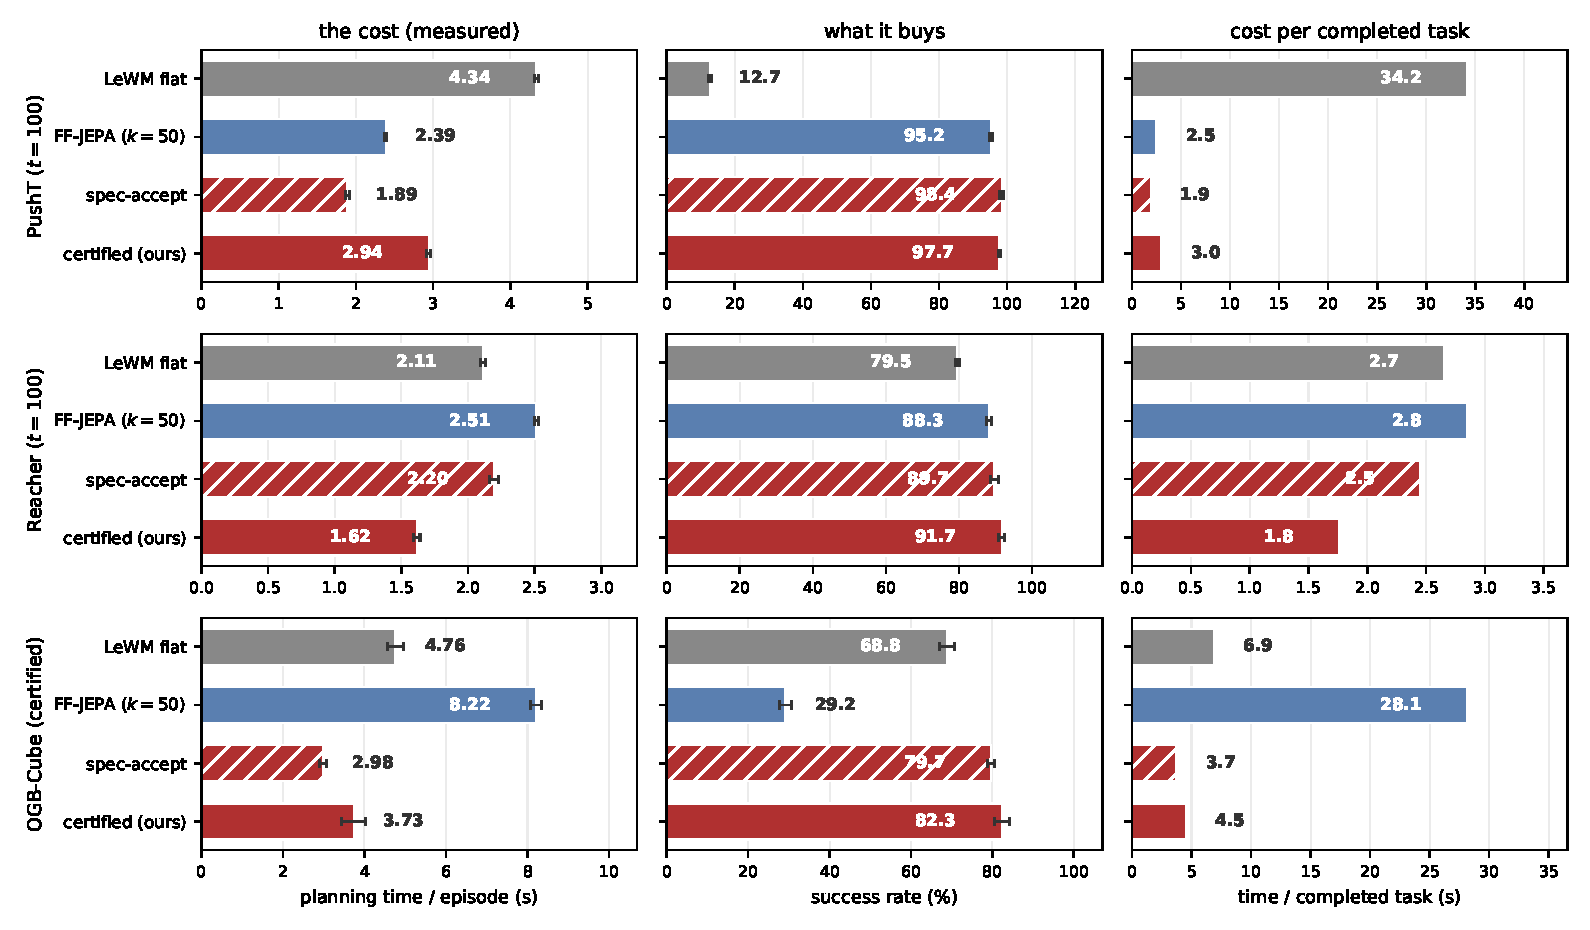
\includegraphics[width=0.82\linewidth]{figs/cost}
\caption{The measured cost story ($5$ seeds; two Cube arms carry $3$--$4$
after node timeouts; error bars $=$ SE; per-episode time includes early
termination on success, the deployment-honest accounting). \textbf{Left:} the
honest overhead, certified spec-accept pays $1.56\times$ spec-accept where
everything drafts (PushT) and is outright \emph{fastest} on Reacher.
\textbf{Middle:} what it buys. \textbf{Right:} time per completed task, the
failing baselines invert from cheapest to most expensive.}
\label{fig:cost}
\end{figure}

\subsection{Certification: the verifier held to account}
\label{sec:results-cert}
The word \emph{certified} is cheap unless the certificate itself is audited;
this subsection does that, pre-registered end to end.

\textbf{Calibration against ground truth.} For every headline serving arm we
replayed each verification event offline (replay mismatches: zero everywhere)
and decoded achieved latent and pursued waypoint to ground-truth state through
a probe gated at held-out $R^{2}\geq0.90$ (pre-frozen conservative-row rule
when probe classes disagree). \Cref{tab:calibration} (\Cref{app:calib}) gives
the operating characteristic at the derived $\tau$, against each environment's
\emph{own success radius}: accepted waypoints are physically within it
$100\%$/$90\%$ of
the time on Cube/PushT; on the two tightest criteria (Reacher $0.05$\,rad,
Two-Room $16$\,px) accepts sit at $80$--$107\%$ of the radius with
$2.5$--$3\times$ separation from rejects, and Reacher's verifier ranks true
angular distance at $\rho=0.978$. The residual false-accepts are
near-boundary: sweeping the readout radius (decisions and $\tau$ fixed),
Reacher's rate falls $0.400\to0.064$ at twice the criterion radius ($0.003$ at
three times) and Two-Room's $0.522\to0.130$ (\Cref{fig:cert-cal},
\Cref{app:calib}). Errors elsewhere are conservative: the verifier errs by
paying an unnecessary re-draft, not by serving a bad waypoint.

\textbf{The derived $\tau$ localizes closed-loop detection.} Displacing every
drafted waypoint by relative noise $\sigma$ and serving through the unchanged
verifier, the call ratio ignites from its banked baseline to total rejection
exactly as $\sigma$ crosses the derived threshold: $0.59\to0.66\to1.00\to1.00$
across $\sigma=0/0.1/0.2/0.4$ (\Cref{fig:cert-decision}, \Cref{app:calib}),
the ignition point our offline derivation predicted before the sweep ran. The
companion prediction failed honestly and is reported: success was flat for
both arms at every $\sigma$, because fresh-draw isotropic jitter is temporally
averaged by \emph{any} consumption policy; verification's success-rate value
is against \emph{autocorrelated} divergence (\Cref{sec:why-verifier}), not
white noise.

\textbf{What the decision carries: rate, not per-event selectivity.} We
pre-registered a matched-rate random-rejection control: an i.i.d.\ coin rejects
at the banked cells' own measured per-event rejection probability
($0.494$/$0.490$ from serving-log counters), everything else byte-identical. The coin \emph{ties} the fixed spec-accept arm on both
$t{=}150$ headline cells ($98.05$ vs.\ $98.14$ PushT; $90.33$ vs.\ $91.11$
Reacher), and a pre-registered dose-response below the matched rate completes
the decomposition: success climbs monotonically with rejection rate on Reacher
($84.6$ at $p{=}0$ to $90.4$ by $p{=}0.25$) and is a step function on PushT
(blind commitment loses $18$pp; $p{=}0.125$ recovers to within $1.2$pp). At
nominal operation, \emph{which} replans are rejected is not load-bearing;
\emph{how often} is. Three things the coin cannot do keep the verifier
essential: its matched rate exists only in hindsight, read off the verifier's
own telemetry; a fixed coin cannot ignite when reality diverges; and its
decisions certify nothing. Verification, on this evidence, is a
\emph{calibrated, adaptive controller of the re-anchoring rate}, and the
paper's mechanism claims are stated at that strength and no more.

\textbf{The serving loop measures its own regime.} Mined over every banked grid
cell ($1{,}525$ log rows), the call ratio falls with goal distance exactly as
the regime map predicts (PushT $0.88\to0.57$, Reacher $0.75\to0.58$ across
$t{=}25\to150$; Two-Room's $0.96$ the registered weak-encoder exception): the
verifier's telemetry is a free per-episode regime diagnostic.

\textbf{The same audit runs at foundation scale.} Applied to V-JEPA 2 ViT-g
pooled latents over $400$ recorded DROID episodes, pre-registered as a
\emph{dataset-pair} characteristic (no serving loop exists there; ground truth
is recorded, not probed), the transferred $\tau{=}0.20$ accepts $85\%$ of
within-episode pairs, rejects $99.9\%$ of cross-episode pairs, and rank-tracks
end-effector distance at $\rho=0.53$, above PushT's own deployed row. The
threshold is metrically \emph{loose} there (median accepted pair $=12.7$\,cm;
DROID defines no task radius), so the row certifies rank sensitivity and
scene discrimination rather than a success-radius guarantee.

\subsection{Held-out environments}
\label{sec:results-heldout}
Two environments were held out until the recipe was frozen. \textbf{Cube}
confirmed its pre-registered bar at $+14.0$pp over the strongest flat (bar
$+5$), the environment's best confirmed number. \textbf{Two-Room}, the
substrate authors' own weakest benchmark, is the modularity test: its encoder
fails the gap precondition outright, the accept test transplants unchanged
into frozen DINOv2 with $\tau$ derived there, and the certified loop recovers
$+15.4$pp at $t{=}75$ (all $12$ seeds, paired $t{\approx}11$, statistically
\emph{at} the measured oracle ceiling) at a protocol anchored to the published
number. The window-rule composite, its switch read off the measured crossover
$[40,50]$, ties the authors' own protocol at $t{=}25$ and never loses to flat;
the compute-matched control recovers $+5.3$pp but certified spec-accept holds
$+10.0$pp above it at less planning compute and $+2\%$ wall-clock. Full arc
in \Cref{app:heldout}.

\section{Analysis: Why It Works}
\label{sec:why}
% The user-designated killer section. Every claim here is a measured
% mechanism, not narration. Target: a reviewer can reconstruct WHEN the
% method will help on an unseen task, and WHY, from this section alone.

\subsection{Verification is regime-dependent, and the regime is predictable}
\label{sec:why-verifier}
We tested verification against its strongest alternative, \emph{blind
commitment} at matched $k$; three regimes give three answers, one theory (full
analysis in \Cref{app:why}). \textbf{Where drafts track reality}
(in-distribution PushT), blind commit-2 ties spec-accept ($65.3$ vs.\ $65.0$)
and verification is idle, \emph{correctly} so: a floor-calibrated verifier
fires only on real divergence. \textbf{Where drafts genuinely diverge}
(exploratory Reacher), re-anchoring is load-bearing: blind commitment loses
$5.9$--$7.6$pp, and the rate-matched control of \Cref{sec:results-cert}
attributes the value to the re-anchoring \emph{rate} the verifier discovers
and holds. \textbf{Where drafts are unconverged} (PushT $k{\le}2$),
floor-calibrated verification backfires exactly as the floor theory predicts,
noise above the floor rejects everything and inherits every-step's churn
($63.5$ vs.\ $55.6$); the derived $k$ rule keeps the operating point off this
cliff. Blindness, by contrast, fails unsignaled in both directions (commit-2
safe on PushT, commit-3 $-18$pp there, any depth loses on Reacher).

\paragraph{The churn thesis.} One mechanism ties these together:
\emph{closed-loop control pays for target consistency; re-drafting injects
churn proportional to draft noise; the consumption policy is churn
management}. Five independent measurements agree: the cadence-isolation
collapse ($-12$pp), the $\gamma$ dose-response, the $S{=}5$ anomaly
(spec-accept \emph{beating} its own every-step reference by $+5$pp), the
$k$-cliff inversion, and the Reacher blind loss.

\paragraph{Drafter stochasticity is load-bearing.}\label{sec:why-spread}
Every operator that collapses drafts toward the conditional mean damages
control despite equal-or-better \emph{offline} fidelity (refinement head that
\emph{halves} offline error: $-11$pp; matched deterministic regressor: $-4.4$
to $-11.7$pp). The $\gamma$-sweep unifies these: SR is non-monotone with the
optimum at native spread ($S{=}25$: $49.0\to\ours{57.9}\to4.7$ across
$\gamma{=}0\to2$; \Cref{app:why}). Control pays for conditional spread near
the training level, in both directions.

\subsection{When drafting pays: the regime map}
\label{sec:why-regime}
Three bounds and one condition, each measured. \textbf{(i) Decomposition tax:}
at short range, ground-truth waypoints tie flat planning ($84.2$ vs.\ $84.0$)
and straight-line waypoints lose monotonically in hop count; no drafter can
beat parity inside the planner's lookahead.
\textbf{(ii) Necessity at range:} the straight-line oracle fails at long range
($33$--$55\%$ vs.\ the drafter's $94.5$); latent geometry is nonlinear, so the
\emph{learned} draft distribution is not replaceable by interpolation.
\textbf{(iii) Data conditionality:} goal-free drafting works exactly when the
data flows toward goals (on expert PushT, conditioning changes nothing; on
exploratory Reacher, goal-free drafting is the random-policy floor,
$8.6$--$11.3\%$ vs.\ $60.6$--$95.1\%$ conditioned). \textbf{(iv) Budget
headroom:} under budget starvation the ordering inverts and flat wins
(\Cref{app:controls}); imperfect waypoints need slack.

The operating rule, stated once: \emph{draft when the goal outruns the planning
window, the goal is inferable from data or conditioning, and the budget affords
imperfect waypoints; plan flat otherwise.} TwoRoom and OGBench-Cube are the
out-of-sample tests, and the scorecard (\Cref{tab:scorecard},
\Cref{app:fulltables}) is $3.5$ of $4$: PushT, Reacher, and TwoRoom as
predicted; Cube the honest half-miss (expert goal-directed data was predicted
sufficient for goal-free drafting and is not), diagnosed and kept in the
scorecard, a rule surviving $3.5/4$ pre-registered predictions with its
failure diagnosed being worth more than an unfalsified one. The $c^{*}$
arbiter (\Cref{sec:method-arbiter}) is the rule's per-episode
operationalization, and \Cref{sec:results-unified} its closed-loop test as a
\emph{policy}.

% ============================================================
% ============================================================
% NEW SECTIONS (post-freeze program, 2026-07-22 -- 07-27).
% Input from main_v2 just before "Negative Results".
% Every closed number here is from an archived pre-registered run;
% \inflight marks batteries whose bars are frozen and running.
% ============================================================

\section{The Verification Gap: Applicability, Measured in Advance}
\label{sec:instrument}

The criterion floor of \Cref{sec:calib-tau} is half of a more general object. The
accept test must separate two distributions computable from cached latents alone:
\emph{equivalence} distances (states one frame apart, arrived, up to task
tolerance) and \emph{hop} distances (states one subgoal interval apart, did not
move). A workable threshold exists iff the interval
\[
\mathcal{G} \;=\; \bigl[\, \mathrm{equiv}\ p_{90},\;\; \mathrm{hop}\ p_{10} \,\bigr]
\]
is non-empty, and $\tau$ must lie inside it. We call $\mathcal{G}$ the
\textbf{verification gap} and compute it for every substrate this paper touches
(\Cref{fig:gap}), one GPU-pass over cached latents, minutes per environment, no
closed-loop rollouts.

% Figure: the verification-gap instrument across nine substrates (pgfplots).
% Input via % Figure: the verification-gap instrument across nine substrates (pgfplots).
% Input via \input{figures/fig_gap_tikz}. Requires pgfplots (compat>=1.16) and
% \definecolor{gapopen}{HTML}{2A78D6} \definecolor{gapmech}{HTML}{EB6834}
% \definecolor{gapdead}{HTML}{E34948} in the preamble.
\begin{figure}[t]
\centering
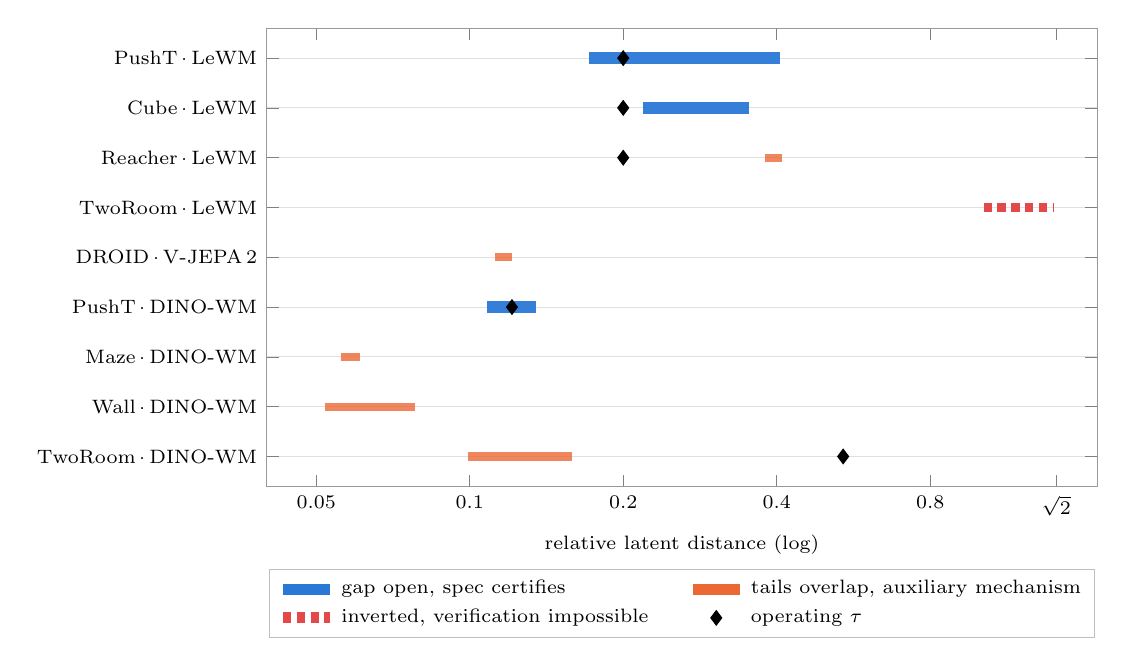
\begin{tikzpicture}
\begin{axis}[
  width=\linewidth, height=7.4cm,
  xmode=log, xmin=0.04, xmax=1.7,
  xtick={0.05,0.1,0.2,0.4,0.8,1.414},
  xticklabels={0.05,0.1,0.2,0.4,0.8,$\sqrt{2}$},
  xlabel={relative latent distance (log)},
  ymin=0.4, ymax=9.6,
  ytick={9,8,7,6,5,4,3,2,1},
  yticklabels={PushT\,·\,LeWM, Cube\,·\,LeWM, Reacher\,·\,LeWM,
               TwoRoom\,·\,LeWM, DROID\,·\,V-JEPA\,2, PushT\,·\,DINO-WM,
               Maze\,·\,DINO-WM, Wall\,·\,DINO-WM, TwoRoom\,·\,DINO-WM},
  y tick label style={font=\scriptsize},
  x tick label style={font=\scriptsize},
  xlabel style={font=\scriptsize},
  axis line style={black!40},
  ymajorgrids, grid style={black!12},
  legend style={font=\scriptsize, at={(0.5,-0.18)}, anchor=north,
                draw=black!25, /tikz/every even column/.append style={column sep=12pt}},
  legend columns=2,
  legend cell align=left,
]
% legend proxies
\addlegendimage{gapopen, line width=4pt}
\addlegendentry{gap open, spec certifies}
\addlegendimage{gapmech, line width=4pt}
\addlegendentry{tails overlap, auxiliary mechanism}
\addlegendimage{gapdead, line width=4pt, densely dashed}
\addlegendentry{inverted, verification impossible}
\addlegendimage{only marks, mark=diamond*, mark size=2.6pt, black}
\addlegendentry{operating $\tau$}

% open gaps [equiv p90 -> hop p10]
\addplot[gapopen, line width=4.5pt, opacity=0.95] coordinates {(0.171,9) (0.406,9)};
\addplot[gapopen, line width=4.5pt, opacity=0.95] coordinates {(0.219,8) (0.353,8)};
\addplot[gapopen, line width=4.5pt, opacity=0.95] coordinates {(0.108,4) (0.135,4)};
% tail overlap (drawn hop p10 -> equiv p90)
\addplot[gapmech, line width=3pt, opacity=0.8] coordinates {(0.379,7) (0.410,7)};
\addplot[gapmech, line width=3pt, opacity=0.8] coordinates {(0.112,5) (0.121,5)};
\addplot[gapmech, line width=3pt, opacity=0.8] coordinates {(0.056,3) (0.061,3)};
\addplot[gapmech, line width=3pt, opacity=0.8] coordinates {(0.052,2) (0.078,2)};
\addplot[gapmech, line width=3pt, opacity=0.8] coordinates {(0.099,1) (0.159,1)};
% inverted (dashed)
\addplot[gapdead, line width=3pt, densely dashed] coordinates {(1.018,6) (1.393,6)};
% taus
\addplot[only marks, mark=diamond*, mark size=2.6pt, black]
  coordinates {(0.20,9) (0.20,8) (0.20,7) (0.121,4) (0.540,1)};
\end{axis}
\end{tikzpicture}
\caption{\textbf{The verification gap across nine substrates.} The verifier must
separate \emph{arrived} (adjacent-frame noise, equiv p90, the criterion floor of
\Cref{sec:calib-tau}) from \emph{did not move} (one subgoal hop, hop p10); the
interval between them is where $\tau$ can operate, computed from cached latents in
minutes. Every closed-loop outcome in this paper matches its row: PushT's in-gap
$\tau$ needed no auxiliary mechanism; Cube's below-gap $\tau$ required the arrival
gate; Reacher's tail overlap required the $c^{*}$ router; TwoRoom-on-LeWM is
inverted at every stride (verification provably cannot operate, even ground-truth
demo waypoints verify $14/113$); DROID's pooled space is degenerate at any $\tau$.
On DINO-WM the instrument ran \emph{before} any closed-loop cell: PushT's gap is
open but the transfer $\tau{=}0.20$ lies above it, so $\tau{=}0.121$ was derived and
frozen; the bottom row shows TwoRoom \emph{cured} of inversion by swapping the
encoder (frozen DINOv2, same pixels), with the learned-lens $\tau$ marked.}
\label{fig:gap}
\end{figure}
. Requires pgfplots (compat>=1.16) and
% \definecolor{gapopen}{HTML}{2A78D6} \definecolor{gapmech}{HTML}{EB6834}
% \definecolor{gapdead}{HTML}{E34948} in the preamble.
\begin{figure}[t]
\centering
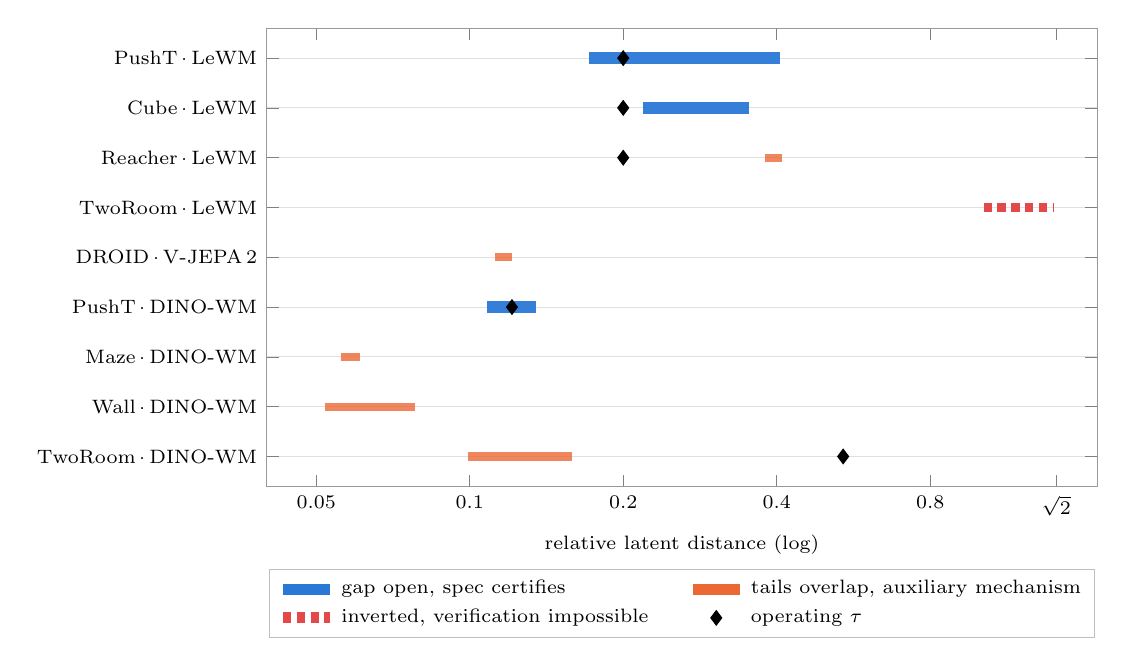
\begin{tikzpicture}
\begin{axis}[
  width=\linewidth, height=7.4cm,
  xmode=log, xmin=0.04, xmax=1.7,
  xtick={0.05,0.1,0.2,0.4,0.8,1.414},
  xticklabels={0.05,0.1,0.2,0.4,0.8,$\sqrt{2}$},
  xlabel={relative latent distance (log)},
  ymin=0.4, ymax=9.6,
  ytick={9,8,7,6,5,4,3,2,1},
  yticklabels={PushT\,·\,LeWM, Cube\,·\,LeWM, Reacher\,·\,LeWM,
               TwoRoom\,·\,LeWM, DROID\,·\,V-JEPA\,2, PushT\,·\,DINO-WM,
               Maze\,·\,DINO-WM, Wall\,·\,DINO-WM, TwoRoom\,·\,DINO-WM},
  y tick label style={font=\scriptsize},
  x tick label style={font=\scriptsize},
  xlabel style={font=\scriptsize},
  axis line style={black!40},
  ymajorgrids, grid style={black!12},
  legend style={font=\scriptsize, at={(0.5,-0.18)}, anchor=north,
                draw=black!25, /tikz/every even column/.append style={column sep=12pt}},
  legend columns=2,
  legend cell align=left,
]
% legend proxies
\addlegendimage{gapopen, line width=4pt}
\addlegendentry{gap open, spec certifies}
\addlegendimage{gapmech, line width=4pt}
\addlegendentry{tails overlap, auxiliary mechanism}
\addlegendimage{gapdead, line width=4pt, densely dashed}
\addlegendentry{inverted, verification impossible}
\addlegendimage{only marks, mark=diamond*, mark size=2.6pt, black}
\addlegendentry{operating $\tau$}

% open gaps [equiv p90 -> hop p10]
\addplot[gapopen, line width=4.5pt, opacity=0.95] coordinates {(0.171,9) (0.406,9)};
\addplot[gapopen, line width=4.5pt, opacity=0.95] coordinates {(0.219,8) (0.353,8)};
\addplot[gapopen, line width=4.5pt, opacity=0.95] coordinates {(0.108,4) (0.135,4)};
% tail overlap (drawn hop p10 -> equiv p90)
\addplot[gapmech, line width=3pt, opacity=0.8] coordinates {(0.379,7) (0.410,7)};
\addplot[gapmech, line width=3pt, opacity=0.8] coordinates {(0.112,5) (0.121,5)};
\addplot[gapmech, line width=3pt, opacity=0.8] coordinates {(0.056,3) (0.061,3)};
\addplot[gapmech, line width=3pt, opacity=0.8] coordinates {(0.052,2) (0.078,2)};
\addplot[gapmech, line width=3pt, opacity=0.8] coordinates {(0.099,1) (0.159,1)};
% inverted (dashed)
\addplot[gapdead, line width=3pt, densely dashed] coordinates {(1.018,6) (1.393,6)};
% taus
\addplot[only marks, mark=diamond*, mark size=2.6pt, black]
  coordinates {(0.20,9) (0.20,8) (0.20,7) (0.121,4) (0.540,1)};
\end{axis}
\end{tikzpicture}
\caption{\textbf{The verification gap across nine substrates.} The verifier must
separate \emph{arrived} (adjacent-frame noise, equiv p90, the criterion floor of
\Cref{sec:calib-tau}) from \emph{did not move} (one subgoal hop, hop p10); the
interval between them is where $\tau$ can operate, computed from cached latents in
minutes. Every closed-loop outcome in this paper matches its row: PushT's in-gap
$\tau$ needed no auxiliary mechanism; Cube's below-gap $\tau$ required the arrival
gate; Reacher's tail overlap required the $c^{*}$ router; TwoRoom-on-LeWM is
inverted at every stride (verification provably cannot operate, even ground-truth
demo waypoints verify $14/113$); DROID's pooled space is degenerate at any $\tau$.
On DINO-WM the instrument ran \emph{before} any closed-loop cell: PushT's gap is
open but the transfer $\tau{=}0.20$ lies above it, so $\tau{=}0.121$ was derived and
frozen; the bottom row shows TwoRoom \emph{cured} of inversion by swapping the
encoder (frozen DINOv2, same pixels), with the learned-lens $\tau$ marked.}
\label{fig:gap}
\end{figure}


\paragraph{One statistic explains every outcome.} PushT's $\tau{=}0.20$ sits inside
its gap $[0.171, 0.406]$: pure spec-accept wins with no auxiliary mechanism
(\Cref{tab:grand}). Cube's gap $[0.219, 0.353]$ sits just \emph{above} the transfer
$\tau$: slight over-rejection, and indeed Cube required the arrival gate. Reacher's
bulks separate $4\times$ but the tails overlap (equiv $p_{90}$ $0.410$ vs.\ hop
$p_{10}$ $0.379$): a noisy verifier, and indeed Reacher required the per-episode
$c^{*}$ router. TwoRoom-on-LeWM is \emph{inverted at every stride}: adjacent
frames read $0.88$ median while unrelated episodes read ${\approx}\sqrt{2}$, the
encoder assigning near-orthogonal codes to distinct positions. No threshold
exists, and the behavioral evidence agrees: a verified oracle serving waypoints the
demonstrator \emph{physically visited} accepted $14/113$ of them. DROID's pooled
space opens no gap at any stride: verification runs degenerate-accept, which is the
honest scope of the scale transplant (\Cref{sec:generality-scale}).

\paragraph{Prescription has a measured boundary.} The instrument's applicability
claim (gap exists $\Rightarrow$ a $\tau$ exists; inverted $\Rightarrow$ verification
cannot operate) is distinct from a stronger prescription we tested and reject: that
the gap \emph{midpoint} is the right $\tau$ and can replace an auxiliary mechanism.
Pre-registered on Cube (8 seeds, gate off, $\tau{=}0.286$ at the midpoint): mechanics
moved as predicted (acceptances ${\sim}3\times$) but SR \emph{fell} to $74.6$ against
a $\ge 78.0$ bar with seed variance tripled: the gate's margin is arrival
protection, not threshold mis-calibration. We therefore claim applicability and
$\tau$-existence, not $\tau$-optimality.

\paragraph{Prospective record.} Three predictions were frozen before their tests and
confirmed: (i) a learned attentive readout cannot open DROID's pooled gap with
$8\times$ data (still closed, width $-0.107$); (ii) $20\times$ data does not repair
the DROID drafter's latent fidelity (no-op ratio $0.39$--$0.48\times$, vs.\ v1's
$0.53$--$0.63\times$); (iii) nor its planning value (paired against v1 across three
budgets: $+0.015/-0.053/+0.074$, all CIs straddling zero). Six further predictions
were frozen before their tests on DINO-WM; their verdicts, including the ones the
serving fault left unresolvable, are reported in \Cref{sec:generality-dinowm}.

\paragraph{When the gap is closed but recoverable: the lens.} Where bulks separate
but tails overlap, a small time-contrastive readout (verifier-side only; world model
and planner untouched) can reopen the interval on held-out episodes: Reacher
$-0.039 \to +0.031$ (derived $\tau{=}0.309$), and on the DINO-WM substrates below,
Maze $-0.006 \to +0.167$, Wall $-0.012 \to +0.146$, TwoRoom-on-DINOv2
$-0.055 \to +0.229$. Two honest boundaries: DROID's pooled space resists the lens at
any tested data scale (information absent from the readout, not mis-read), and an
open lens gap is an \emph{offline} statement: closed-loop, the Reacher lens
traded short-horizon SR ($-4.5$/$-2.5$pp at $t{=}25/50$) for verification
efficiency (call ratio $0.63 \to 0.55$); its closed-loop value is tested
pre-registered on Wall below.

% ============================================================
\section{Generality: A Second Architecture and a Scale Transplant}
\label{sec:generality}

The results of \Cref{sec:results} live on one stack. This section transplants the
method twice, to a second full planning architecture where closed-loop success is
measurable, and to a $55\times$ larger world model where it is not, and lets the
instrument of \Cref{sec:instrument} make its predictions \emph{first}.

\subsection{DINO-WM: derive-first on an architecture adopted mid-project}
\label{sec:generality-dinowm}

DINO-WM \citep{dinowm} plans with MPC-CEM over frozen DINOv2 patch features, a
task-agnostic encoder, unlike LeWM's task-trained one, and therefore the harder
test of the gap's portability. We reproduce its released PushT protocol as the
anchor (flat success $86\%$ at $n{=}50$, seed $99$, vs.\ the paper's $90\%$; our run
caps MPC at the environment's 300-step episode budget), then run the instrument
before any spec-accept cell: PushT's gap is \emph{open} at the natural hop but the
LeWM-transfer $\tau{=}0.20$ sits \emph{above} it, the instrument's first
$\tau$-mis-calibration call; so $\tau{=}0.121$ is derived and the following are
frozen (\texttt{docs/dinowm\_prereg.md}) before execution: \textbf{P1} certified
spec-accept at $\tau{=}0.121$ within $2$pp of flat; \textbf{P2} $\tau{=}0.20$ runs
degenerate-accept; \textbf{P3} Maze/Wall (tail-overlap rows) underperform at any
fixed $\tau$; \textbf{P4} Wall recovers under the lens verifier; \textbf{P5} at
$\mathrm{goal}_H{=}15$, where the drafted block spans the goal distance exactly, the
spec-vs-flat margin improves on its short-horizon value. The transplanted drafter is
the first in this program to beat the no-op reference on a video-feature substrate
(no-op ratio $1.11/1.22/1.31\times$ at block positions $1/2/3$).

Verdicts, reported exactly as they fell. \textbf{P3 confirmed}, the cleanest
prospective hit in the program: Wall at the fixed transfer $\tau$ scores $0.685$
against flat's $1.00$, a $31$pp underperformance the instrument called before the
run. \textbf{P4 unavailable}: the Wall lens never opened a gap at the serving hop,
so no $\tau$ could be derived and the arm was not run, reported rather than
improvised. \textbf{P1, P2, and P5 are confounded and remain open}: across three
independent batteries the flat arms are healthy ($0.82$--$0.88$) while every
spec-accept arm scores near zero with one signature (the drafter passes its offline
gates and beats the no-op reference, yet served waypoints produce no progress),
which indicates an unresolved fault in our DINO-WM serving integration rather than
a verdict on the predictions; we decline to claim them in either direction, and the
predictions stay frozen. Point-maze remains prediction-only (its environment
requires mujoco-py + d4rl).

\subsection{TwoRoom: the scope condition is an encoder property, and repairable}
\label{sec:generality-tworoom}

TwoRoom-on-LeWM is this paper's cleanest impossibility (\Cref{sec:instrument}):
inverted gap, verifier rejecting reality itself, ground-truth waypoints
\emph{halving} flat's success because planning optimizes the same broken metric. The
instrument localizes the failure to the encoder, which makes a causal test
available: push the \emph{same pixels} through frozen DINOv2. The saturation cures:
adjacent-frame distance drops $0.876 \to 0.081$, hops and cross-episode
distances scale properly again, and the substrate lands in the recoverable
tail-overlap class, where the lens opens a usable gap ($+0.229$, derived
$\tau{=}0.540$). The scope condition is not ``TwoRoom is hard'': it is a measurable
property of the encoder's metric, diagnosed in advance, and repaired by a component
swap the instrument itself prescribed.

The closed-loop completion on this substrate (a DINO-WM world model trained on
TwoRoom, drafted arm under the lens verifier) was cut at the program's
pre-declared deadline before its evaluation harness was complete; the encoder-swap
cure above is the measured claim, and the closed-loop arm remains a frozen
prediction. The LeWM-side closed loop, however, did complete
(\Cref{sec:results-heldout}): certifying TwoRoom in frozen DINOv2 while the
planner consumes LeWM latents recovers $+15.4$pp at range, the same
component-swap prescription executed on the verifier alone.

\subsection{V-JEPA 2: what transfers at $55\times$ scale, and what cannot be known offline}
\label{sec:generality-scale}

Transplanted to V-JEPA~2's 1B action-conditioned model (token-grid targets served to
the upstream CEM unmodified), the \emph{mechanism} carries: the certified source runs
end-to-end, and the verifier constant transfers ($\tau{=}0.20$ against measured
single-replan floors of $0.06$--$0.10$). Three things do not, and we report them as
the scale boundary. The planner certificate $c^{*}$ carries no discriminative signal
on this substrate (three independent measurements; a router built on it routes
$0/36$ anchors to flat). The drafter is not rescued by data ($20\times$: predictions
(ii)--(iii) above). And planning \emph{quality} cannot be honestly adjudicated
offline at all: there is no simulator for a real-robot DROID model, in-model scoring
is circular (the model grades plans that may exploit its own errors), and the
demonstration-agreement instrument fails its own sanity checks at $n{=}36$ paired
anchors (flat's agreement ${\approx}0$ and not improving with $16\times$ budget; a
straight-line interpolation outscoring both planners). An exploratory
$15\times$-compute result did not survive this powered pre-registered replication
and is retired accordingly; closed-loop evaluation at scale is future work requiring
hardware, not more offline instruments.

\paragraph{Concurrent work.} SAGE \citep{sage} (July 2026) independently reports that
drafted subgoal latents repair long-horizon myopia on LeWM, converging evidence
for the premise, but consumes its drafts open-loop: no reality-verification, no
applicability instrument, one architecture. TRM \citep{trm} repairs latent-metric
failures with reachability-based metrics, the training-time complement to our
verifier-side lens; its LeWM-vs-PLDM TwoRoom comparison independently supports the
encoder-property reading of \Cref{sec:generality-tworoom}. Our contribution remains
the certificate and the instrument: \emph{when} a drafted plan can be trusted, and
\emph{whether} a given stack can support the trust test at all.


% ============================================================
\section{Discussion and Conclusion}
\label{sec:discussion}
\textbf{Limitations.} (i) FF-JEPA released no code; our configuration is a
principled reconstruction certified by closed-loop anchors
(\Cref{app:repro}). (ii) The $\tau$/$k$ derivations carry two retrospective
validations plus two prospective confirmations; the $\tau$ rule met its
measured Cube scope boundary and fell back to the transferred default. (iii)
The criterion-floor rule is well-posed only when the success criterion covers
the observed scene; under partial observation a scope guard selects the
threshold basis (Cube). (iv) Drafting's value is \emph{conditional}
(\Cref{sec:why-regime}). (v) The \degc{20}/\degc{5} mapping is inferred from
empirical alignment; cross-paper comparisons are marked accordingly. (vi) The
compute claim is a drafter-side NFE claim with its denominator stated;
horizon populations are never spliced.
(vii) The arbiter's routing guarantee is \emph{empirical}: $c^{*}$ inherits
any world-model mis-calibration (degrading softly to the routed parent), the
policy \emph{allocates} capability rather than creating it, and under partial
observation it reads as per-episode solvability.

\label{sec:conclusion}
\textbf{Conclusion.} A planner can trust a drafted plan exactly as long as
reality confirms it; the threshold for ``confirms'' is a measured property of
the encoder, not a hyperparameter. Certified spec-accept turns that into one
policy winning all eleven pre-registered cells at $1.9$--$2.4$ drafter
evaluations per replan; the verification gap makes the precondition
measurable in advance ($+15.4$pp on Two-Room when it fails and is repaired);
any world model that plans by rollout can grade its own homework.

\bibliography{references}
\bibliographystyle{iclr2027_conference}

% ============================================================
\appendix\label{appendixstart}

\section{Full Result Tables}
\label{app:fulltables}
This appendix collects the full tables summarized in the main text: the
spec-accept pseudocode, the configuration policy, the published-protocol
comparison, the fixed-population horizon spine, the certified-policy table with
its complete routing analysis, and the regime-map scorecard.

\begin{algorithm}[h]
\small
\caption{Spec-accept: reality-verified speculative consumption (one env; run per env).}
\label{alg:specaccept}
\begin{algorithmic}[1]
\Require frozen encoder $E$, drafter $G$ (block size $N$, $k$ DDIM steps), controller
CEM, threshold $\tau$; horizon RH$\,{=}\,S/5$
\State $\mathrm{block}\gets G(E(o_0);\,k)$;\quad $j\gets 1$;\quad $w\gets \mathrm{block}[0]$
\Comment{initial draft; $j$ indexes the served position}
\For{each replan boundary with achieved observation $o$}
  \State $z\gets E(o)$
  \If{$j<N$ \textbf{and} $\|z-w\|/\|z\| \le \tau$}
     \Comment{reality confirms the plan, accept, no diffusion call}
     \State $w\gets \mathrm{block}[j]$;\quad $j\gets j+1$
  \Else
     \Comment{reality diverged (or block exhausted), re-anchor}
     \State $\mathrm{block}\gets G(z;\,k)$;\quad $w\gets \mathrm{block}[0]$;\quad $j\gets 1$
  \EndIf
  \State execute CEM toward $w$ for RH action blocks
\EndFor
\end{algorithmic}
\end{algorithm}

% Figure: the certified spec-accept loop (TikZ). Input from main via
% % Figure: the certified spec-accept loop (TikZ). Input from main via
% % Figure: the certified spec-accept loop (TikZ). Input from main via
% \input{figures/fig_method_tikz}. Requires tikz + libraries loaded in preamble:
% \usetikzlibrary{arrows.meta,positioning,shapes.geometric,calc}
\begin{figure}[t]
\centering
\resizebox{0.86\linewidth}{!}{%
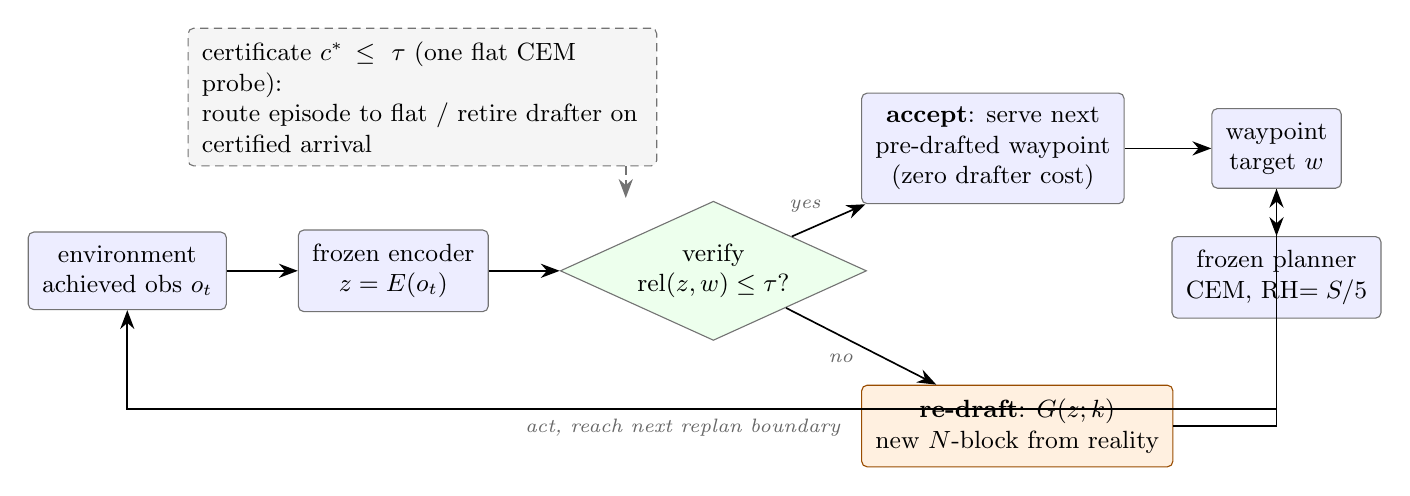
\begin{tikzpicture}[
  font=\small,
  node distance=6mm and 9mm,
  box/.style={draw=black!55, rounded corners=2pt, align=center,
              inner sep=5pt, minimum height=8mm},
  frozen/.style={box, fill=blue!7},
  paid/.style={box, fill=orange!12, draw=orange!60!black},
  verify/.style={diamond, draw=black!55, fill=green!7, align=center,
                 inner sep=2pt, aspect=2.2},
  cert/.style={box, fill=black!4, densely dashed},
  arr/.style={-{Stealth[length=2.4mm]}, semithick},
  lbl/.style={font=\scriptsize\itshape, text=black!60},
]
% main loop
\node[frozen] (env) {environment\\achieved obs $o_t$};
\node[frozen, right=of env] (enc) {frozen encoder\\$z=E(o_t)$};
\node[verify, right=of enc] (ver) {verify\\$\mathrm{rel}(z,w)\le\tau$?};
\node[frozen, above right=4mm and 9mm of ver] (accept)
  {\textbf{accept}: serve next\\pre-drafted waypoint\\(zero drafter cost)};
\node[paid, below right=10mm and 9mm of ver] (draft)
  {\textbf{re-draft}: $G(z;k)$\\new $N$-block from reality};
\node[frozen, right=of accept, xshift=2mm] (target) {waypoint\\target $w$};
\node[frozen, below=of target] (cem) {frozen planner\\CEM, RH$=S/5$};

\draw[arr] (env) -- (enc);
\draw[arr] (enc) -- (ver);
\draw[arr] (ver) -- node[lbl, above left=-1pt]{yes} (accept);
\draw[arr] (ver) -- node[lbl, below left=-1pt]{no} (draft);
\draw[arr] (accept) -- (target);
\draw[arr] (draft) -| (target);
\draw[arr] (target) -- (cem);
\draw[arr] (cem.south) |- ++(-2.0,-1.15) -| node[lbl, pos=0.22, below]{act, reach next replan boundary} (env.south);

% certificate rail (kept clear of the accept node: anchored over env/enc only)
\node[cert, above=8mm of enc.north west, anchor=south west, xshift=-14mm,
      text width=5.6cm, align=left] (cstar)
  {certificate $c^{*}\!\le\tau$ (one flat CEM probe):\\
   route episode to flat / retire drafter on\\certified arrival};
\draw[arr, densely dashed, black!55] (cstar.south east) ++(-4mm,0) -- ++(0,-4mm);
\end{tikzpicture}%
}
\caption{\textbf{Certified spec-accept.} A drafted $N$-block is consumed waypoint by
waypoint; at every replan boundary the \emph{achieved} latent is verified against
the waypoint just pursued. Within $\tau$, the next pre-drafted waypoint is served
at zero drafter cost; otherwise the block is re-drafted from reality. Encoder,
planner, and world model stay frozen (blue); the drafter (orange) is the only paid
component, and the planner's own certificate $c^{*}$ (dashed) decides per episode
and per replan whether drafting is needed at all. $\tau$ is derived, not tuned
(\Cref{sec:calib-tau}).}
\label{fig:method}
\end{figure}
. Requires tikz + libraries loaded in preamble:
% \usetikzlibrary{arrows.meta,positioning,shapes.geometric,calc}
\begin{figure}[t]
\centering
\resizebox{0.86\linewidth}{!}{%
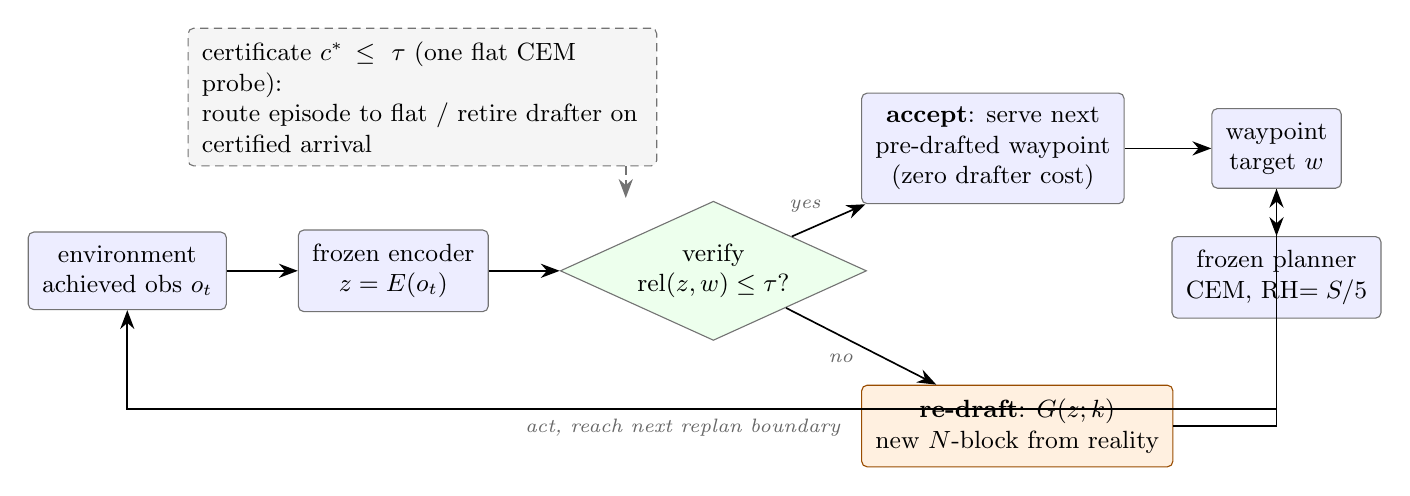
\begin{tikzpicture}[
  font=\small,
  node distance=6mm and 9mm,
  box/.style={draw=black!55, rounded corners=2pt, align=center,
              inner sep=5pt, minimum height=8mm},
  frozen/.style={box, fill=blue!7},
  paid/.style={box, fill=orange!12, draw=orange!60!black},
  verify/.style={diamond, draw=black!55, fill=green!7, align=center,
                 inner sep=2pt, aspect=2.2},
  cert/.style={box, fill=black!4, densely dashed},
  arr/.style={-{Stealth[length=2.4mm]}, semithick},
  lbl/.style={font=\scriptsize\itshape, text=black!60},
]
% main loop
\node[frozen] (env) {environment\\achieved obs $o_t$};
\node[frozen, right=of env] (enc) {frozen encoder\\$z=E(o_t)$};
\node[verify, right=of enc] (ver) {verify\\$\mathrm{rel}(z,w)\le\tau$?};
\node[frozen, above right=4mm and 9mm of ver] (accept)
  {\textbf{accept}: serve next\\pre-drafted waypoint\\(zero drafter cost)};
\node[paid, below right=10mm and 9mm of ver] (draft)
  {\textbf{re-draft}: $G(z;k)$\\new $N$-block from reality};
\node[frozen, right=of accept, xshift=2mm] (target) {waypoint\\target $w$};
\node[frozen, below=of target] (cem) {frozen planner\\CEM, RH$=S/5$};

\draw[arr] (env) -- (enc);
\draw[arr] (enc) -- (ver);
\draw[arr] (ver) -- node[lbl, above left=-1pt]{yes} (accept);
\draw[arr] (ver) -- node[lbl, below left=-1pt]{no} (draft);
\draw[arr] (accept) -- (target);
\draw[arr] (draft) -| (target);
\draw[arr] (target) -- (cem);
\draw[arr] (cem.south) |- ++(-2.0,-1.15) -| node[lbl, pos=0.22, below]{act, reach next replan boundary} (env.south);

% certificate rail (kept clear of the accept node: anchored over env/enc only)
\node[cert, above=8mm of enc.north west, anchor=south west, xshift=-14mm,
      text width=5.6cm, align=left] (cstar)
  {certificate $c^{*}\!\le\tau$ (one flat CEM probe):\\
   route episode to flat / retire drafter on\\certified arrival};
\draw[arr, densely dashed, black!55] (cstar.south east) ++(-4mm,0) -- ++(0,-4mm);
\end{tikzpicture}%
}
\caption{\textbf{Certified spec-accept.} A drafted $N$-block is consumed waypoint by
waypoint; at every replan boundary the \emph{achieved} latent is verified against
the waypoint just pursued. Within $\tau$, the next pre-drafted waypoint is served
at zero drafter cost; otherwise the block is re-drafted from reality. Encoder,
planner, and world model stay frozen (blue); the drafter (orange) is the only paid
component, and the planner's own certificate $c^{*}$ (dashed) decides per episode
and per replan whether drafting is needed at all. $\tau$ is derived, not tuned
(\Cref{sec:calib-tau}).}
\label{fig:method}
\end{figure}
. Requires tikz + libraries loaded in preamble:
% \usetikzlibrary{arrows.meta,positioning,shapes.geometric,calc}
\begin{figure}[t]
\centering
\resizebox{0.86\linewidth}{!}{%
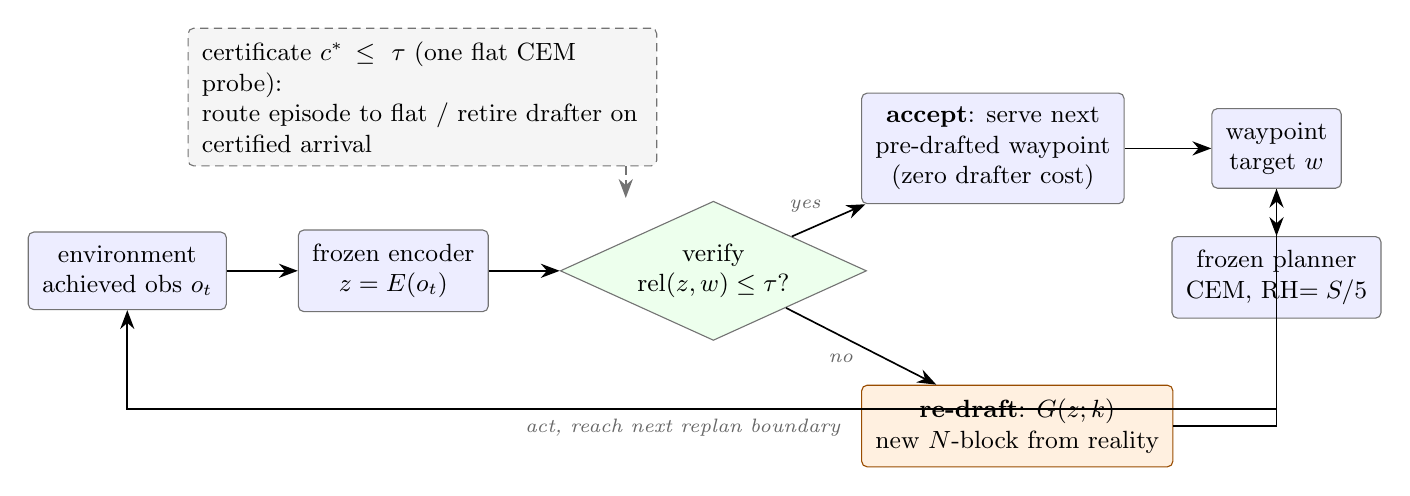
\begin{tikzpicture}[
  font=\small,
  node distance=6mm and 9mm,
  box/.style={draw=black!55, rounded corners=2pt, align=center,
              inner sep=5pt, minimum height=8mm},
  frozen/.style={box, fill=blue!7},
  paid/.style={box, fill=orange!12, draw=orange!60!black},
  verify/.style={diamond, draw=black!55, fill=green!7, align=center,
                 inner sep=2pt, aspect=2.2},
  cert/.style={box, fill=black!4, densely dashed},
  arr/.style={-{Stealth[length=2.4mm]}, semithick},
  lbl/.style={font=\scriptsize\itshape, text=black!60},
]
% main loop
\node[frozen] (env) {environment\\achieved obs $o_t$};
\node[frozen, right=of env] (enc) {frozen encoder\\$z=E(o_t)$};
\node[verify, right=of enc] (ver) {verify\\$\mathrm{rel}(z,w)\le\tau$?};
\node[frozen, above right=4mm and 9mm of ver] (accept)
  {\textbf{accept}: serve next\\pre-drafted waypoint\\(zero drafter cost)};
\node[paid, below right=10mm and 9mm of ver] (draft)
  {\textbf{re-draft}: $G(z;k)$\\new $N$-block from reality};
\node[frozen, right=of accept, xshift=2mm] (target) {waypoint\\target $w$};
\node[frozen, below=of target] (cem) {frozen planner\\CEM, RH$=S/5$};

\draw[arr] (env) -- (enc);
\draw[arr] (enc) -- (ver);
\draw[arr] (ver) -- node[lbl, above left=-1pt]{yes} (accept);
\draw[arr] (ver) -- node[lbl, below left=-1pt]{no} (draft);
\draw[arr] (accept) -- (target);
\draw[arr] (draft) -| (target);
\draw[arr] (target) -- (cem);
\draw[arr] (cem.south) |- ++(-2.0,-1.15) -| node[lbl, pos=0.22, below]{act, reach next replan boundary} (env.south);

% certificate rail (kept clear of the accept node: anchored over env/enc only)
\node[cert, above=8mm of enc.north west, anchor=south west, xshift=-14mm,
      text width=5.6cm, align=left] (cstar)
  {certificate $c^{*}\!\le\tau$ (one flat CEM probe):\\
   route episode to flat / retire drafter on\\certified arrival};
\draw[arr, densely dashed, black!55] (cstar.south east) ++(-4mm,0) -- ++(0,-4mm);
\end{tikzpicture}%
}
\caption{\textbf{Certified spec-accept.} A drafted $N$-block is consumed waypoint by
waypoint; at every replan boundary the \emph{achieved} latent is verified against
the waypoint just pursued. Within $\tau$, the next pre-drafted waypoint is served
at zero drafter cost; otherwise the block is re-drafted from reality. Encoder,
planner, and world model stay frozen (blue); the drafter (orange) is the only paid
component, and the planner's own certificate $c^{*}$ (dashed) decides per episode
and per replan whether drafting is needed at all. $\tau$ is derived, not tuned
(\Cref{sec:calib-tau}).}
\label{fig:method}
\end{figure}


\begin{table}[h]
\centering
\small
\caption{Configuration policy. $\tau$ and $k$ are measured properties of the stack;
$S$ is tuned and reported as a result.}
\label{tab:config}
\setlength{\tabcolsep}{4pt}
\begin{tabular}{llp{6.6cm}}
\toprule
knob & value (dev envs) & basis \\
\midrule
$\tau$ (acceptance threshold) & $0.20$ & \emph{derived}: the encoder's criterion
floor, the latent distance at which the benchmark's own success tolerance stops
distinguishing states (\Cref{sec:calib-tau}); validated retrospectively against
closed-loop grids on both dev environments and an episode-disjoint split \\
$k$ (DDIM steps per draft) & $3$ (PushT) / any (Reacher) & \emph{derived}: the
sampler's convergence point, measured by repeat-draw dispersion
(\Cref{sec:calib-k}); on PushT the derived $k{=}3$ was never swept and was confirmed
prospectively; the inherited $k{=}50$ is image-domain convention,
${\sim}17\times$ overpriced \\
$S$ (subgoal scale) & per env, tuned & swept on dev envs; both show an interior
optimum at $S{=}10$ at short range (\Cref{sec:calib-scale}). Pre-registered rule for
held-out envs: $S{=}10$ zero-shot as the primary arm (transfer of the dev-env
optimum), gated by an offline displacement sanity probe ($\mathrm{disp}(S)$ well
above the criterion floor); an optional $S\in\{5,25\}$ secondary curve is reported
as a finding, never used for selection \\
$\gamma$ (draft noise scale) & $1$ (native) & not a knob: swept once as a mechanism
experiment (\Cref{sec:why}) \\
\bottomrule
\end{tabular}
\end{table}

\begin{table}[h]
\centering
\small
\caption{PushT, the published system's own protocols (\degc{20}; short/long
$n{=}1024$, random-init $n{=}1024$, 4 seeds each). Spec-accept at the derived config
($\tau{=}0.20$, $k{=}3$). $^{p}$published (LeWM/FF-JEPA Table I); every ``our'' row is
4 seeds on the certified pipeline.}
\label{tab:headline2}
\begin{tabular}{lcccc}
\toprule
& short $t{=}25$ & long $t{=}75$ & random init & NFE/replan \\
\midrule
LeWM flat                    & 94.5$^{p}$ & 3.5$^{p}$ & 0.0$^{p}$ & 0 \\
FF-JEPA (published)          & 96.1$^{p}$ & 91.8$^{p}$ & 82.4$^{p}$ & 50 \\
FF-JEPA config (our run)     & 94.8 & 90.1 & 98.8 & 50 \\
Ours: $S^{*}$ every-step     & \ours{99.4} & \ours{97.9} & \ours{100.0} & 50 \\
Ours: $+$ spec-accept        & 98.7 & 97.2 & \ours{100.0} & \ours{1.9} \\
\bottomrule
\end{tabular}
\end{table}

\begin{table}[h]
\centering
\small
\setlength{\tabcolsep}{6pt}
\caption{The spine: fixed-population horizon sweeps (\degc{20} / joint criterion,
$n{=}512$/cell). Within each sub-table, identical episodes at every offset; the two
Reacher populations (max-offset-100 for $t{\le}100$, max-offset-150 for $t{\ge}125$)
have different eligible episodes by construction and are never merged into a single
row; $t{=}100$ appears in both and differs (e.g.\ our $S{=}10$ arm: $90.8$ vs.\
$94.5$), a transparent measure of that sensitivity. Every-step arms sample at
$k{=}50$; spec-accept at the derived configuration. All Reacher drafters are
goal-conditioned (one identical recipe per scale); the goal-free recipe measures at
the random-policy floor here ($8.6$--$11.3$, \Cref{sec:why-regime}) and is omitted.
Flat shown at RH$=$5, its strongest configuration at range; a faster flat (RH$=$2)
is stronger at short horizon ($t{=}25$: $95.7$), which only widens the short-range
decomposition tax that bounds every waypoint method there (\Cref{sec:why-regime}).
$^{\ast}$Reacher spec cells on the max-offset-100 population predate the
$k$-derivation and ran $k{=}8$; the max-offset-150 cells use the derived $k{=}4$;
both track their every-step reference within noise.}
\label{tab:spine}

\vspace{2pt}
\textbf{(a) PushT} \quad \emph{success-filtered fixed population, budget $2t$, 2 seeds}

\vspace{2pt}
\begin{tabular}{llccccc}
\toprule
& configuration & $t{=}25$ & $t{=}50$ & $t{=}75$ & $t{=}100$ & $t{=}150$ \\
\midrule
flat (goal image)   & RH$=$5                          & 98.1 & 60.4 & 42.6 & 12.7 & 2.7 \\
FF-JEPA config      & $S{=}25$, every-step            & 99.0 & 94.1 & 95.9 & 95.7 & 93.9 \\
ours, every-step    & $S{=}10$                        & 99.6 & \ours{99.0} & 98.1 & \ours{98.1} & \ours{98.4} \\
ours, spec-accept   & $S{=}10$, $\tau{=}0.20$, $k{=}3$ & \ours{99.6} & 97.9 & \ours{98.8} & 97.3 & 98.1 \\
\midrule
\multicolumn{2}{l}{gap (best ours $-$ flat)} & $+1.5$ & $+38.6$ & $+56.2$ & $+85.4$ & $+95.7$ \\
\bottomrule
\end{tabular}

\vspace{8pt}
\textbf{(b) Reacher, native$\to$crossover} \quad \emph{max-offset-100 population,
budget $2t$, 4 seeds}

\vspace{2pt}
\begin{tabular}{llcccc}
\toprule
& configuration & $t{=}25$ & $t{=}50$ & $t{=}75$ & $t{=}100$ \\
\midrule
flat (goal image)   & RH$=$5                             & \ours{83.2} & \ours{91.8} & 89.1 & 83.2 \\
FF-JEPA config      & $S{=}25$, every-step               & 55.5 & 78.9 & 89.8 & 89.5 \\
ours, every-step    & $S{=}10$                           & 59.8 & 79.7 & \ours{90.2} & \ours{90.8} \\
ours, spec-accept   & $S{=}10$, $\tau{=}0.20$, $k{=}8^{\ast}$ & 54.3 & 79.3 & 90.0 & \ours{91.0} \\
\bottomrule
\end{tabular}

\vspace{8pt}
\textbf{(c) Reacher, extended range and scale} \quad \emph{max-offset-150
population, budget $2t$, 4 seeds}

\vspace{2pt}
\begin{tabular}{llccc}
\toprule
& configuration & $t{=}100$ & $t{=}125$ & $t{=}150$ \\
\midrule
flat (goal image)   & RH$=$5                             & 83.2 & 81.4 & 76.0 \\
drafted, every-step & $S{=}5$                            & 91.2 & 93.0 & 93.0 \\
drafted, every-step & $S{=}15$                           & 93.9 & 93.8 & 95.5 \\
FF-JEPA config      & $S{=}25$, every-step               & 93.6 & 91.8 & 92.6 \\
ours, every-step    & $S{=}10$                           & 94.5 & 93.2 & 95.1 \\
ours, spec-accept   & $S{=}10$, $\tau{=}0.20$, $k{=}4$    & \ours{95.5} & \ours{95.5} & \ours{95.7} \\
\midrule
\multicolumn{2}{l}{gap (best ours $-$ flat)} & $+11.3$ & $+14.1$ & $+19.7$ \\
\bottomrule
\end{tabular}
\end{table}

\begin{figure}[h]
\centering
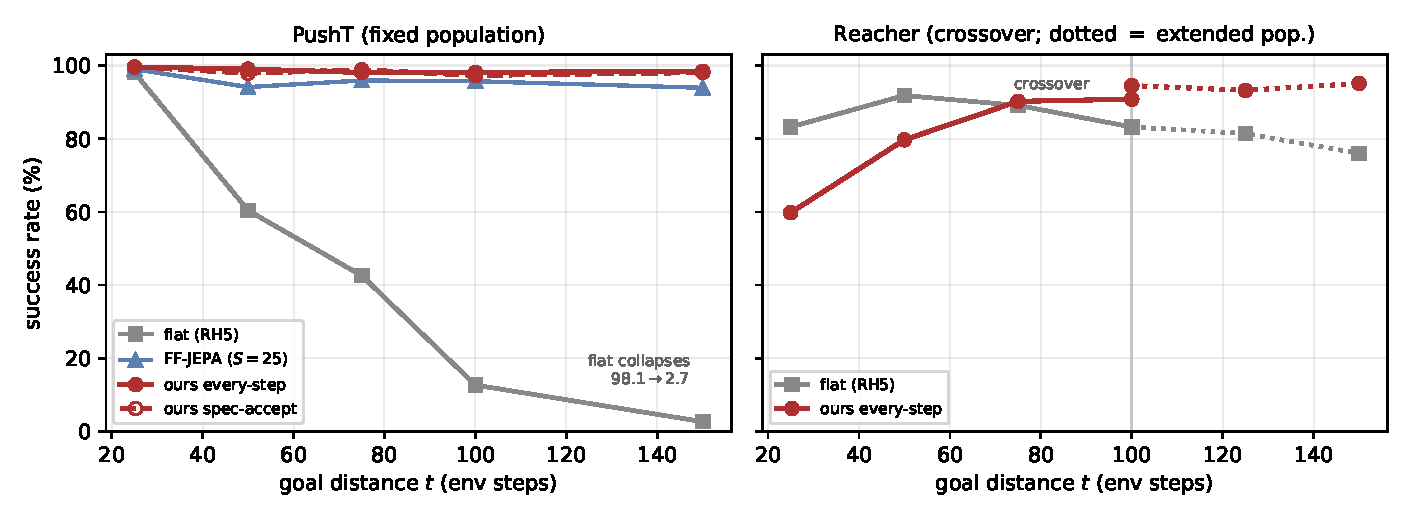
\includegraphics[width=\linewidth]{figs/spine}
\caption{The spine: success vs.\ goal distance, flat family
vs.\ drafted arms, on the fixed-population sweeps of \Cref{tab:spine}. \textbf{PushT
(left):} flat planning collapses monotonically ($98.1\to2.7$) while every drafted arm
holds ${\sim}98$; spec-accept (open circles) tracks every-step. \textbf{Reacher
(right):} the mechanism as a crossover, flat leads inside the planner's lookahead,
the $S{=}10$ drafter draws level by $t{\approx}75$ and leads thereafter. The two
Reacher populations (solid $=$ max-offset-100 for $t{\le}100$; dotted $=$
max-offset-150 for $t{\ge}100$) are plotted without splicing, both $t{=}100$ values
shown. Cube contributes a single horizon by construction (single-transport task)
and is tabulated in \Cref{tab:cube}; TwoRoom's crossover arc is
\Cref{fig:tworoom-crossover}.}
\label{fig:spine}
\end{figure}

\begin{table}[h]
\centering
\small
\caption{Certified spec-accept on Reacher (fresh confirmation population, budget
$2t$, $n{=}128$, pooled over 8 seeds $=$ $1024$ episodes/cell; per-cell SE
$0.2$--$0.7$pp; joint criterion). The policy composes the routed episodes: each
episode executed once, under the arm chosen from its start state by $c^{*}$ at frozen
$\tau{=}0.20$. The full policy applies the rule at both scopes
(\Cref{sec:method-arbiter}); the routing-only row is the ablation with mid-episode
retirement disabled, isolating each scope's contribution. Pre-registered bar: the
policy $\ge$ the strongest flat arm at every $t$, scored on the declared seeds
42--45, met $4/4$; the extension seeds 46--49 were declared before their results and
are pooled without selection.}
\label{tab:unified}
\begin{tabular}{lcccc}
\toprule
& $t{=}25$ & $t{=}50$ & $t{=}100$ & $t{=}150$ \\
\midrule
flat, RH$=$2                  & 95.7 & 88.8 & 60.8 & 58.3 \\
flat, RH$=$5                  & 83.0 & 93.0 & 79.2 & 75.9 \\
spec-accept (fixed arm)       & 57.3 & 78.7 & 88.2 & \ours{91.1} \\
routing only (ablation)       & 98.2 & 94.9 & 90.7 & 89.9 \\
\ours{certified spec-accept (full)} & \ours{98.7} & \ours{96.3} & \ours{92.3} & 90.1 \\
\midrule
margin vs.\ strongest flat    & $+3.0$ & $+3.3$ & $+13.1$ & $+14.3$ \\
\bottomrule
\end{tabular}
\end{table}

\paragraph{Full routing analysis (\Cref{sec:results-unified}).}
Against our own fixed spec-accept arm the policy wins outright at $t{\le}100$
and sits $-1.0$pp behind at $t{=}150$, at the edge of the declared $\pm1$pp
band, persistent across all eight seeds, and reported as such. Routing
composition shifts exactly as the regime map predicts (flat-routed fraction
$99\%\to75\%$ over $t{=}25\to150$), and the certificate's selection is nearly
pure: episodes routed to short-window flat succeed at $96.7$--$100\%$ at
\emph{every} horizon and every seed, including $t{=}150$ where flat's
population average is $58.3\%$. Two closures on the routing rule itself, both
computed \emph{exactly} offline from dumped per-episode outcomes (no new
rollouts). \emph{Threshold robustness:} the composite SR is flat across
$\tau\in[0.15,0.40]$ at every horizon (identical to $0.1$pp in most cells;
only $\tau{=}0.10$ under-fires), the router's plateau is wider than the
verifier's, and the shared $\tau{=}0.20$ sits mid-plateau. \emph{Allocation
ceiling:} against the per-episode oracle mix (route each episode to whichever
arm succeeded, the ceiling of any router), the certificate captures
$97$--$99\%$ of the achievable gain at every horizon. \emph{Why both hold, the
certificate separates:} pooled over all horizons and seeds ($2{,}048$
episodes), $c^{*}$ is bimodal: $70\%$ of episodes sit below $0.15$, where flat
succeeds $98.7\%$; $24\%$ sit above $1.0$, where flat succeeds $17.7\%$ and
spec-accept $81.7\%$; and $6$ episodes in two thousand fall anywhere between.
$P(\text{flat succeeds})$ drops $81$ points across the threshold, and $\tau$
sits in a near-empty valley between two clean clusters, which is why selection
is nearly pure, why any threshold in $[0.15,0.40]$ makes essentially identical
decisions, and why one number can serve verifier, router, and retirement
without per-use tuning. The compute-matched control: doubling flat's CEM
samples (a strict upper bound on the measured $1.58\times$) at $t{\ge}100$
rescues nothing on PushT ($12.7{\to}15.0$ at $t{=}100$; $3.1{\to}2.9$ at
$t{=}150$) and on Reacher buys flat-RH5 $+1$--$2$pp and flat-RH2
$+10$--$12$pp, our frozen prediction (``no material rescue'') was right for
three arms of four and too strong for the under-optimized short window,
reported as-is. On PushT the composite additionally beats the pure spec spine
outright at $t{=}25$ ($99.8$, including a $256/256$ seed) and $t{=}100$; the
full policy (retirement enabled) reads the same ($97.3$--$99.6$, $5/5$), and
at $t{\ge}100$ the composite \emph{is} the drafting leg, since zero episodes
route to flat.

\begin{table}[h]
\centering
\small
\setlength{\tabcolsep}{4pt}
\caption{The regime-map scorecard: the rule's three conditions per environment,
its prediction, and what the batteries measured. Predictions for TwoRoom and Cube
were registered before their runs; the Cube inferability miss is kept in the
scorecard and diagnosed (arrival is absent from always-in-motion training
segments, \Cref{sec:results-heldout}).}
\label{tab:scorecard}
\begin{tabular}{lcccp{4.1cm}}
\toprule
env & beyond window? & goal inferable? & headroom? & outcome vs.\ prediction \\
\midrule
PushT   & yes ($t{\ge}50$) & yes (goal-free) & yes & drafting wins, predicted \\
Reacher & at $t{\gtrsim}75$ & conditioned only & yes & crossover at $t{\approx}75$, predicted \\
TwoRoom & yes & \textbf{no} (goal-free) & yes & goal-free fails, predicted; verify in external space \\
Cube    & yes & \emph{miss}: conditioning required & yes & wins once conditioned $+$ arrival \\
\bottomrule
\end{tabular}
\end{table}

\section{Calibration: Full Grids and Validation}
\label{app:calib}
The closed-loop validation grids behind \Cref{sec:calib}, and the calibration
table and figures behind \Cref{sec:results-cert}. The $\tau$-grids were run
independently of the floor measurement and agree with it three ways
retrospectively (optima on the floors; plateau ordering by floor; below-floor
false-reject signature) plus one prospective check (the band widening with
$S$, \Cref{sec:calib-tau}).

\begin{table}[h]
\centering
\small
\caption{The verifier's operating characteristic at the derived $\tau$, per
environment, from replayed serving decisions ($991$--$3{,}552$ events/env) decoded
to ground-truth state. FA/FR $=$ false-accept/false-reject rates at the
environment's own success-criterion radius; acc p50 $=$ median physical distance of
accepted waypoints vs.\ that radius. Conservative probe row quoted where classes
disagree (pre-frozen rule); Reacher uses the registered circular (sin/cos) probe
after the raw-angle probe failed its gate, both outcomes reported.}
\label{tab:calibration}
\begin{tabular}{lccccc}
\toprule
& probe $R^{2}$ & $\rho$(rel, state) & FA & FR & acc p50 / radius \\
\midrule
Cube & .992 & .72 & .000 & .59 & .013 / .04 \\
PushT & .983 & .49 & .102 & .58 & 8.7 / 20 \\
Reacher (circ.) & .997 & \textbf{.978} & .400 & .045 & .040 / .05 \\
Two-Room & .998 & .36 & .522 & .13 & 17.2 / 16 \\
\bottomrule
\end{tabular}
\end{table}

\begin{table}[h]
\centering
\small
\caption{The floor measurements (accept-test units, $n{=}436$--$512$ pairs/anchors).
Derived $\tau$ = the criterion floor; the value used everywhere in this paper
($0.20$) sits on both environments' floors, and the environments' \emph{different}
floors predict their different closed-loop plateaus (\Cref{tab:taugrid}). The
strict \degc{5} criterion variant, which exists only for PushT, reads p50
$0.173$ / p90 $0.718$.}
\label{tab:floor}
\begin{tabular}{lcccc}
\toprule
& \multicolumn{2}{c}{PushT} & \multicolumn{2}{c}{Reacher} \\
\cmidrule(lr){2-3}\cmidrule(lr){4-5}
& p50 & p90 & p50 & p90 \\
\midrule
temporal floor (consecutive frames)     & 0.080 & 0.152 & 0.223 & 0.428 \\
criterion floor (success-equivalent)    & 0.233 & 0.843 & 0.106 & 0.153 \\
\midrule
reference: true $S{=}10$ displacement   & 0.700 & 1.085 & 0.866 & 1.351 \\
\bottomrule
\end{tabular}
\end{table}

\begin{table}[h]
\centering
\small
\caption{Closed-loop $\tau$-grids, the \emph{validation} of the derived threshold
(\degc{20} / joint criterion; call ratio in parentheses). PushT anchors on the
unfiltered (harder) fixed populations; Reacher on the max-offset-100 fixed
population; $n{=}512$/cell except val split ($n{=}512$, 2 seeds). SR flat inside
each environment's floor band, calls monotone, degradation onset ordered by the
floors (\Cref{tab:floor}).}
\label{tab:taugrid}
\begin{tabular}{lcccccc}
\toprule
& $\tau{=}0.10$ & $0.15$ & $0.20$ & $0.25$ & $0.30$ & $0.40$ \\
\midrule
PushT $t{=}100$, $k{=}4$        & 64.1 (.87) & --- & 65.0 (.58) & --- & 65.0 (.47) & --- \\
PushT val split $t{=}150$, $k{=}8$ & --- & 63.5 (.61) & 64.5 (.50) & 63.7 (.45) & 63.7 (.42) & --- \\
Reacher $t{=}100$, $k{=}4$      & 95.9 (.84) & --- & 95.5 (.63) & --- & 94.1 (.52) & 90.2 (.46) \\
\bottomrule
\end{tabular}
\end{table}

\begin{table}[h]
\centering
\small
\caption{Subgoal-scale sweep, every-step drafting (\degc{20} / joint criterion,
$n{=}512$--$1024$/cell, 4 seeds). PushT short on the paper-matched success-filtered
population; PushT $t{=}150$ on the unfiltered fixed population (harder; compare
within-row only). Interior optimum at $S{=}10$ on three of four rows; flat at Reacher
long range.}
\label{tab:scurve}
\begin{tabular}{lcccc}
\toprule
& $S{=}5$ & $S{=}10$ & $S{=}15$ & $S{=}25$ (native) \\
\midrule
PushT short $t{=}25$        & 98.6 & \ours{99.4} & 98.4 & 94.8 \\
PushT long $t{=}150$        & 55.3 & \ours{59.6} & 58.3 & 55.9 \\
Reacher short $t{=}25$      & 52.5 & \ours{60.6} & 54.5 & 53.9 \\
Reacher long $t{=}100/150$  & 91.2\,/\,93.0 & 94.5\,/\,95.1 & 93.9\,/\,\ours{95.5} & 93.6\,/\,92.6 \\
\bottomrule
\end{tabular}
\end{table}

\begin{figure}[h]
\centering
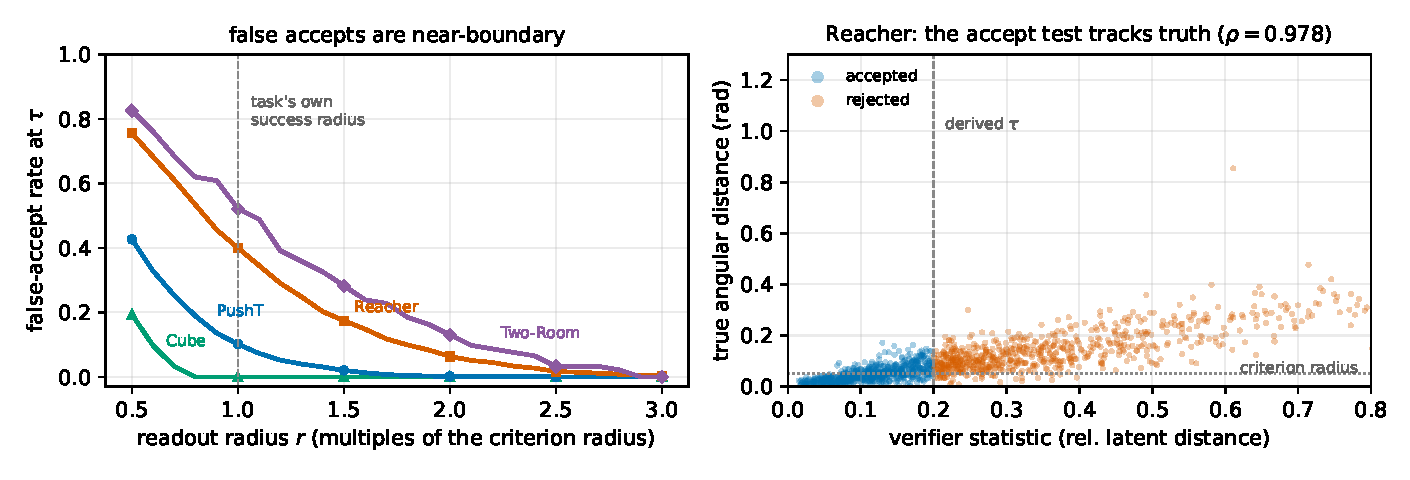
\includegraphics[width=\linewidth]{figs/cert_cal}
\caption{\textbf{Calibration against ground truth.} \textbf{Left:} false-accept
rate as the readout radius sweeps around each task's own success radius
(decisions and $\tau$ fixed): the residual false accepts are near-boundary,
collapsing to $0.064$/$0.130$ at twice the Reacher/Two-Room radii and to
$0.003$ at three times on Reacher; Cube is already exact at its criterion.
\textbf{Right:} the Reacher operating scatter, replayed serving decisions
against true wrapped angular distance: the latent test ranks physical truth at
$\rho=0.978$, with the derived $\tau$ separating the two populations.}
\label{fig:cert-cal}
\end{figure}

\begin{figure}[h]
\centering
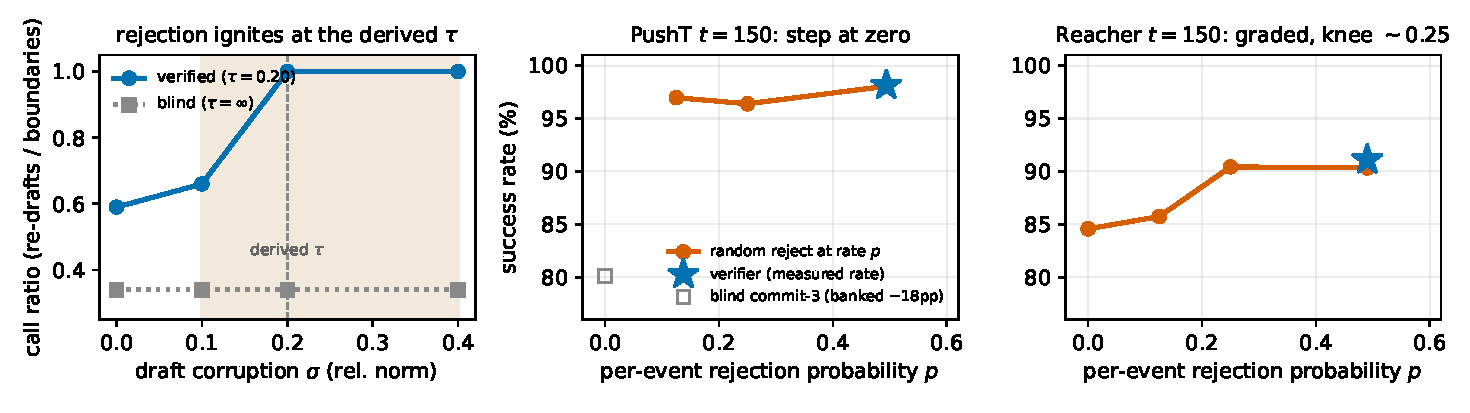
\includegraphics[width=\linewidth]{figs/cert_decision}
\caption{\textbf{What the accept decision buys, measured three ways.}
\textbf{Left:} under drafter corruption the verifier's call ratio ignites from
its banked baseline to total rejection exactly as $\sigma$ crosses the
offline-derived $\tau$ (shaded: the pre-registered $[\tau/2,2\tau]$ band); blind
consumption sits at its mechanical floor throughout. \textbf{Middle, right:} the
pre-registered rejection-rate dose-response. Random rejection at the verifier's
own measured rate (star) ties it on both headline cells; below that rate,
success is a step function on PushT (blind commit-3 loses $18$pp; $p{=}0.125$
already recovers) and graded on Reacher (knee ${\sim}0.25$). The rate is
load-bearing; per-event selectivity is not, and the rate itself is knowable only
from the verifier's telemetry.}
\label{fig:cert-decision}
\end{figure}

\section{Mechanism Analysis in Full}
\label{app:why}
The complete blind-commitment analysis behind \Cref{sec:why-verifier}, and the
full stochasticity dose-response behind \Cref{sec:why-spread}.

\textbf{Where drafts track reality, verification is idle, and correctly so.}
In-distribution PushT (expert data), blind commit-2 ties spec-accept at both
anchors ($65.3$ vs.\ $65.0$ at $t{=}100$; $58.1$ vs.\ $58.9$ at $t{=}150$; $k{=}4$)
at call ratio $0.50$ vs.\ spec's $0.53$--$0.63$. A verifier calibrated at the floor
fires only on real divergence; when there is none, it is behaviorally equivalent to
not checking. This tie is a \emph{prediction} of the floor calibration, not a
failure of it.

\textbf{Where drafts genuinely diverge, re-anchoring is load-bearing, and the
verifier is what sets its rate.} On Reacher (exploratory data; drafts inherit the
collection policy's meanders), the verifier fires constantly (call ratio $0.62$),
and removing re-anchoring costs real success: blind commitment scores $87.9/89.8$
at $t{=}100/150$ vs.\ spec-accept's $95.5/95.7$, a $+5.9$--$7.6$pp gap. The
certification battery (\Cref{sec:results-cert}) sharpens the attribution: a
rate-matched random-rejection control ties the verifier here, so the value at
nominal operation is the re-anchoring \emph{rate} the verifier discovers and
holds, not the identity of the rejected replans; the rejections land exactly
where the regime map's data-conditionality leg (\Cref{sec:why-regime}) predicts
plans and reality part ways.

\textbf{Where drafts are \emph{unconverged}, naive verification backfires, as the
floor theory itself explains.} At the PushT $k{\leq}2$ cliff, blind commit-2
scores $63.5$ (plateau quality at $1$ NFE/replan) while spec-accept falls to $55.6$:
with sampler noise far above the floor (\Cref{sec:calib-k}: dispersion $0.65$ vs.\
floor $0.23$), a floor-calibrated $\tau$ rejects everything and inherits
every-step's real failure mode, \emph{churn}, a freshly re-sampled noisy target
every replan that CEM chases. Committed positions of one block are internally
consistent, so commitment beats re-drafting there. The derived $k$ rule keeps the
operating point off this cliff, and we report the cell as the boundary of validity
of floor-calibrated verification rather than hide it.

\textbf{Why not just always commit blindly?} Blind commitment carries a hidden
hyperparameter with its own cliff: depth. Commit-2 is safe on PushT; commit-3 loses
$18$pp there (\Cref{sec:negatives}) and blind commitment loses $6$--$8$pp on Reacher
at the depth its block provides, and blindness has no signal for which regime it
is in. The dose-response of \Cref{sec:results-cert} maps the cliff precisely: the
loss is confined to (near-)zero re-anchoring rates, and a \emph{random} rejection
ladder recovers success once its rate reaches the knee, but that ladder's rate is
only knowable from the verifier's own telemetry, cannot ignite under divergence,
and certifies nothing. Spec-accept subsumes the whole family ($\tau{\to}0$ is
every-step, $\tau{\to}\infty$ is blind), the measured floor picks the operating
point, and the realized call ratio is a free, per-episode regime diagnostic:
${\approx}0.5$ means verification is idle insurance; ${<}0.7$ and falling means it
is earning its keep.

\textbf{The full $\gamma$ dose-response.} Sweeping the sampler's noise scale at
fixed everything ($\gamma\in\{0,0.25,\ldots,1.5,2\}$, both scales, long-horizon
anchor): SR is non-monotone with the optimum at native spread, $S{=}25$:
$49.0\to53.7\to55.1\to56.1\to\ours{57.9}\to56.1\to28.7\to4.7$ across
$\gamma{=}0\to2$; $S{=}10$ traces the same shape with a gentler low side
($56.6$ at $\gamma{=}0$, peak $59.1$--$59.4$ at $\gamma{=}1$--$1.25$, $8.4$ at
$\gamma{=}2$). A deterministic regressor matching the drafter's offline error
loses $4.4$--$11.7$pp closed-loop.

\section{The Verification Gap Across Substrates, and Generality in Full}
\label{app:generality}
The nine-substrate gap figure behind \Cref{sec:instrument}, and the complete
transplant narratives behind \Cref{sec:generality}.

% Figure: the verification-gap instrument across nine substrates (pgfplots).
% Input via % Figure: the verification-gap instrument across nine substrates (pgfplots).
% Input via % Figure: the verification-gap instrument across nine substrates (pgfplots).
% Input via \input{figures/fig_gap_tikz}. Requires pgfplots (compat>=1.16) and
% \definecolor{gapopen}{HTML}{2A78D6} \definecolor{gapmech}{HTML}{EB6834}
% \definecolor{gapdead}{HTML}{E34948} in the preamble.
\begin{figure}[t]
\centering
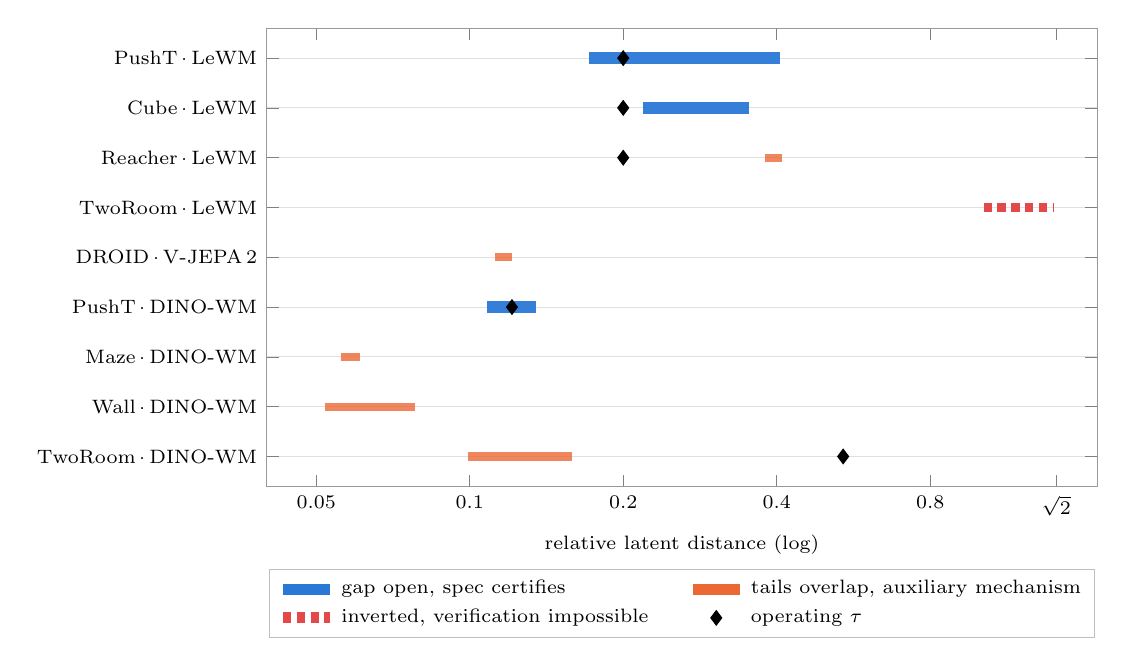
\begin{tikzpicture}
\begin{axis}[
  width=\linewidth, height=7.4cm,
  xmode=log, xmin=0.04, xmax=1.7,
  xtick={0.05,0.1,0.2,0.4,0.8,1.414},
  xticklabels={0.05,0.1,0.2,0.4,0.8,$\sqrt{2}$},
  xlabel={relative latent distance (log)},
  ymin=0.4, ymax=9.6,
  ytick={9,8,7,6,5,4,3,2,1},
  yticklabels={PushT\,·\,LeWM, Cube\,·\,LeWM, Reacher\,·\,LeWM,
               TwoRoom\,·\,LeWM, DROID\,·\,V-JEPA\,2, PushT\,·\,DINO-WM,
               Maze\,·\,DINO-WM, Wall\,·\,DINO-WM, TwoRoom\,·\,DINO-WM},
  y tick label style={font=\scriptsize},
  x tick label style={font=\scriptsize},
  xlabel style={font=\scriptsize},
  axis line style={black!40},
  ymajorgrids, grid style={black!12},
  legend style={font=\scriptsize, at={(0.5,-0.18)}, anchor=north,
                draw=black!25, /tikz/every even column/.append style={column sep=12pt}},
  legend columns=2,
  legend cell align=left,
]
% legend proxies
\addlegendimage{gapopen, line width=4pt}
\addlegendentry{gap open, spec certifies}
\addlegendimage{gapmech, line width=4pt}
\addlegendentry{tails overlap, auxiliary mechanism}
\addlegendimage{gapdead, line width=4pt, densely dashed}
\addlegendentry{inverted, verification impossible}
\addlegendimage{only marks, mark=diamond*, mark size=2.6pt, black}
\addlegendentry{operating $\tau$}

% open gaps [equiv p90 -> hop p10]
\addplot[gapopen, line width=4.5pt, opacity=0.95] coordinates {(0.171,9) (0.406,9)};
\addplot[gapopen, line width=4.5pt, opacity=0.95] coordinates {(0.219,8) (0.353,8)};
\addplot[gapopen, line width=4.5pt, opacity=0.95] coordinates {(0.108,4) (0.135,4)};
% tail overlap (drawn hop p10 -> equiv p90)
\addplot[gapmech, line width=3pt, opacity=0.8] coordinates {(0.379,7) (0.410,7)};
\addplot[gapmech, line width=3pt, opacity=0.8] coordinates {(0.112,5) (0.121,5)};
\addplot[gapmech, line width=3pt, opacity=0.8] coordinates {(0.056,3) (0.061,3)};
\addplot[gapmech, line width=3pt, opacity=0.8] coordinates {(0.052,2) (0.078,2)};
\addplot[gapmech, line width=3pt, opacity=0.8] coordinates {(0.099,1) (0.159,1)};
% inverted (dashed)
\addplot[gapdead, line width=3pt, densely dashed] coordinates {(1.018,6) (1.393,6)};
% taus
\addplot[only marks, mark=diamond*, mark size=2.6pt, black]
  coordinates {(0.20,9) (0.20,8) (0.20,7) (0.121,4) (0.540,1)};
\end{axis}
\end{tikzpicture}
\caption{\textbf{The verification gap across nine substrates.} The verifier must
separate \emph{arrived} (adjacent-frame noise, equiv p90, the criterion floor of
\Cref{sec:calib-tau}) from \emph{did not move} (one subgoal hop, hop p10); the
interval between them is where $\tau$ can operate, computed from cached latents in
minutes. Every closed-loop outcome in this paper matches its row: PushT's in-gap
$\tau$ needed no auxiliary mechanism; Cube's below-gap $\tau$ required the arrival
gate; Reacher's tail overlap required the $c^{*}$ router; TwoRoom-on-LeWM is
inverted at every stride (verification provably cannot operate, even ground-truth
demo waypoints verify $14/113$); DROID's pooled space is degenerate at any $\tau$.
On DINO-WM the instrument ran \emph{before} any closed-loop cell: PushT's gap is
open but the transfer $\tau{=}0.20$ lies above it, so $\tau{=}0.121$ was derived and
frozen; the bottom row shows TwoRoom \emph{cured} of inversion by swapping the
encoder (frozen DINOv2, same pixels), with the learned-lens $\tau$ marked.}
\label{fig:gap}
\end{figure}
. Requires pgfplots (compat>=1.16) and
% \definecolor{gapopen}{HTML}{2A78D6} \definecolor{gapmech}{HTML}{EB6834}
% \definecolor{gapdead}{HTML}{E34948} in the preamble.
\begin{figure}[t]
\centering
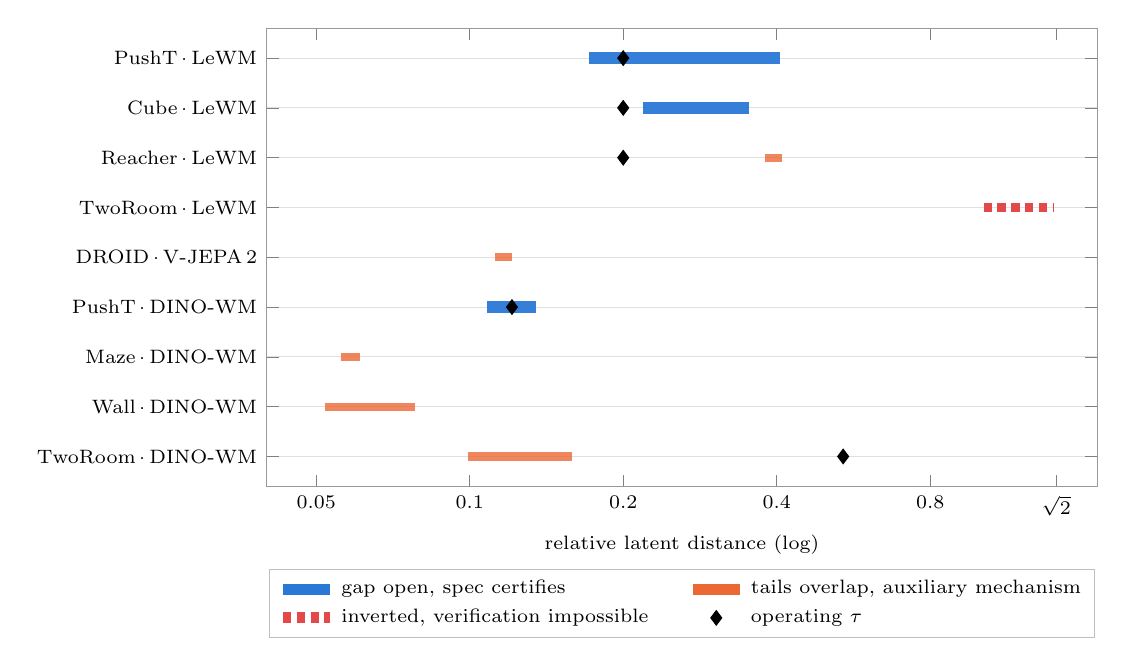
\begin{tikzpicture}
\begin{axis}[
  width=\linewidth, height=7.4cm,
  xmode=log, xmin=0.04, xmax=1.7,
  xtick={0.05,0.1,0.2,0.4,0.8,1.414},
  xticklabels={0.05,0.1,0.2,0.4,0.8,$\sqrt{2}$},
  xlabel={relative latent distance (log)},
  ymin=0.4, ymax=9.6,
  ytick={9,8,7,6,5,4,3,2,1},
  yticklabels={PushT\,·\,LeWM, Cube\,·\,LeWM, Reacher\,·\,LeWM,
               TwoRoom\,·\,LeWM, DROID\,·\,V-JEPA\,2, PushT\,·\,DINO-WM,
               Maze\,·\,DINO-WM, Wall\,·\,DINO-WM, TwoRoom\,·\,DINO-WM},
  y tick label style={font=\scriptsize},
  x tick label style={font=\scriptsize},
  xlabel style={font=\scriptsize},
  axis line style={black!40},
  ymajorgrids, grid style={black!12},
  legend style={font=\scriptsize, at={(0.5,-0.18)}, anchor=north,
                draw=black!25, /tikz/every even column/.append style={column sep=12pt}},
  legend columns=2,
  legend cell align=left,
]
% legend proxies
\addlegendimage{gapopen, line width=4pt}
\addlegendentry{gap open, spec certifies}
\addlegendimage{gapmech, line width=4pt}
\addlegendentry{tails overlap, auxiliary mechanism}
\addlegendimage{gapdead, line width=4pt, densely dashed}
\addlegendentry{inverted, verification impossible}
\addlegendimage{only marks, mark=diamond*, mark size=2.6pt, black}
\addlegendentry{operating $\tau$}

% open gaps [equiv p90 -> hop p10]
\addplot[gapopen, line width=4.5pt, opacity=0.95] coordinates {(0.171,9) (0.406,9)};
\addplot[gapopen, line width=4.5pt, opacity=0.95] coordinates {(0.219,8) (0.353,8)};
\addplot[gapopen, line width=4.5pt, opacity=0.95] coordinates {(0.108,4) (0.135,4)};
% tail overlap (drawn hop p10 -> equiv p90)
\addplot[gapmech, line width=3pt, opacity=0.8] coordinates {(0.379,7) (0.410,7)};
\addplot[gapmech, line width=3pt, opacity=0.8] coordinates {(0.112,5) (0.121,5)};
\addplot[gapmech, line width=3pt, opacity=0.8] coordinates {(0.056,3) (0.061,3)};
\addplot[gapmech, line width=3pt, opacity=0.8] coordinates {(0.052,2) (0.078,2)};
\addplot[gapmech, line width=3pt, opacity=0.8] coordinates {(0.099,1) (0.159,1)};
% inverted (dashed)
\addplot[gapdead, line width=3pt, densely dashed] coordinates {(1.018,6) (1.393,6)};
% taus
\addplot[only marks, mark=diamond*, mark size=2.6pt, black]
  coordinates {(0.20,9) (0.20,8) (0.20,7) (0.121,4) (0.540,1)};
\end{axis}
\end{tikzpicture}
\caption{\textbf{The verification gap across nine substrates.} The verifier must
separate \emph{arrived} (adjacent-frame noise, equiv p90, the criterion floor of
\Cref{sec:calib-tau}) from \emph{did not move} (one subgoal hop, hop p10); the
interval between them is where $\tau$ can operate, computed from cached latents in
minutes. Every closed-loop outcome in this paper matches its row: PushT's in-gap
$\tau$ needed no auxiliary mechanism; Cube's below-gap $\tau$ required the arrival
gate; Reacher's tail overlap required the $c^{*}$ router; TwoRoom-on-LeWM is
inverted at every stride (verification provably cannot operate, even ground-truth
demo waypoints verify $14/113$); DROID's pooled space is degenerate at any $\tau$.
On DINO-WM the instrument ran \emph{before} any closed-loop cell: PushT's gap is
open but the transfer $\tau{=}0.20$ lies above it, so $\tau{=}0.121$ was derived and
frozen; the bottom row shows TwoRoom \emph{cured} of inversion by swapping the
encoder (frozen DINOv2, same pixels), with the learned-lens $\tau$ marked.}
\label{fig:gap}
\end{figure}
. Requires pgfplots (compat>=1.16) and
% \definecolor{gapopen}{HTML}{2A78D6} \definecolor{gapmech}{HTML}{EB6834}
% \definecolor{gapdead}{HTML}{E34948} in the preamble.
\begin{figure}[t]
\centering
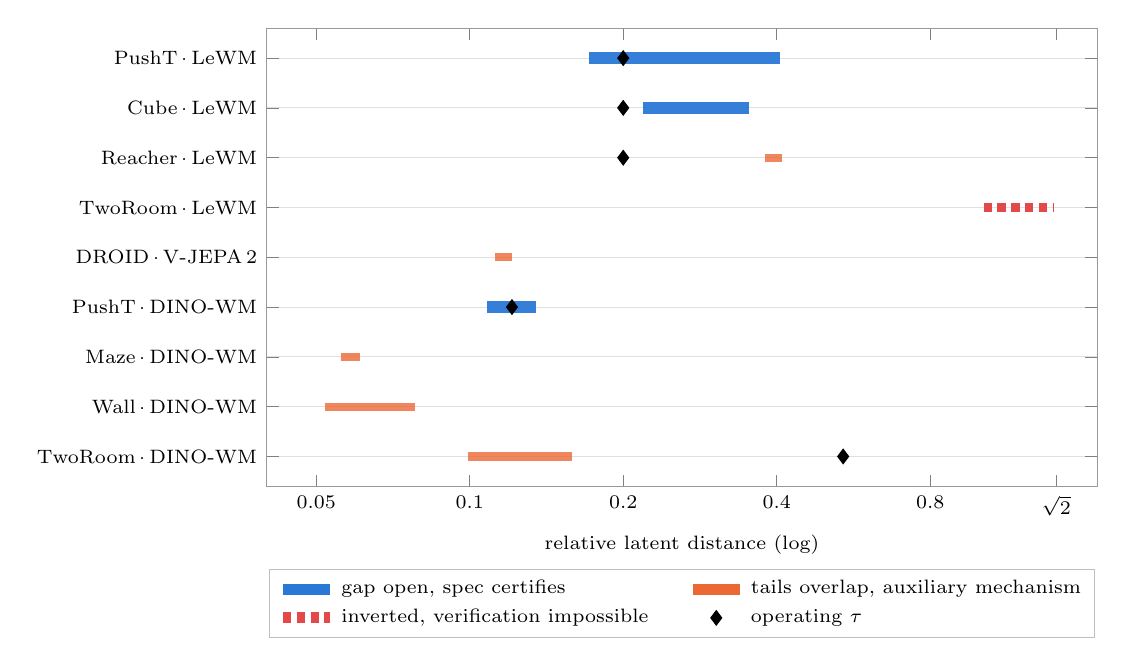
\begin{tikzpicture}
\begin{axis}[
  width=\linewidth, height=7.4cm,
  xmode=log, xmin=0.04, xmax=1.7,
  xtick={0.05,0.1,0.2,0.4,0.8,1.414},
  xticklabels={0.05,0.1,0.2,0.4,0.8,$\sqrt{2}$},
  xlabel={relative latent distance (log)},
  ymin=0.4, ymax=9.6,
  ytick={9,8,7,6,5,4,3,2,1},
  yticklabels={PushT\,·\,LeWM, Cube\,·\,LeWM, Reacher\,·\,LeWM,
               TwoRoom\,·\,LeWM, DROID\,·\,V-JEPA\,2, PushT\,·\,DINO-WM,
               Maze\,·\,DINO-WM, Wall\,·\,DINO-WM, TwoRoom\,·\,DINO-WM},
  y tick label style={font=\scriptsize},
  x tick label style={font=\scriptsize},
  xlabel style={font=\scriptsize},
  axis line style={black!40},
  ymajorgrids, grid style={black!12},
  legend style={font=\scriptsize, at={(0.5,-0.18)}, anchor=north,
                draw=black!25, /tikz/every even column/.append style={column sep=12pt}},
  legend columns=2,
  legend cell align=left,
]
% legend proxies
\addlegendimage{gapopen, line width=4pt}
\addlegendentry{gap open, spec certifies}
\addlegendimage{gapmech, line width=4pt}
\addlegendentry{tails overlap, auxiliary mechanism}
\addlegendimage{gapdead, line width=4pt, densely dashed}
\addlegendentry{inverted, verification impossible}
\addlegendimage{only marks, mark=diamond*, mark size=2.6pt, black}
\addlegendentry{operating $\tau$}

% open gaps [equiv p90 -> hop p10]
\addplot[gapopen, line width=4.5pt, opacity=0.95] coordinates {(0.171,9) (0.406,9)};
\addplot[gapopen, line width=4.5pt, opacity=0.95] coordinates {(0.219,8) (0.353,8)};
\addplot[gapopen, line width=4.5pt, opacity=0.95] coordinates {(0.108,4) (0.135,4)};
% tail overlap (drawn hop p10 -> equiv p90)
\addplot[gapmech, line width=3pt, opacity=0.8] coordinates {(0.379,7) (0.410,7)};
\addplot[gapmech, line width=3pt, opacity=0.8] coordinates {(0.112,5) (0.121,5)};
\addplot[gapmech, line width=3pt, opacity=0.8] coordinates {(0.056,3) (0.061,3)};
\addplot[gapmech, line width=3pt, opacity=0.8] coordinates {(0.052,2) (0.078,2)};
\addplot[gapmech, line width=3pt, opacity=0.8] coordinates {(0.099,1) (0.159,1)};
% inverted (dashed)
\addplot[gapdead, line width=3pt, densely dashed] coordinates {(1.018,6) (1.393,6)};
% taus
\addplot[only marks, mark=diamond*, mark size=2.6pt, black]
  coordinates {(0.20,9) (0.20,8) (0.20,7) (0.121,4) (0.540,1)};
\end{axis}
\end{tikzpicture}
\caption{\textbf{The verification gap across nine substrates.} The verifier must
separate \emph{arrived} (adjacent-frame noise, equiv p90, the criterion floor of
\Cref{sec:calib-tau}) from \emph{did not move} (one subgoal hop, hop p10); the
interval between them is where $\tau$ can operate, computed from cached latents in
minutes. Every closed-loop outcome in this paper matches its row: PushT's in-gap
$\tau$ needed no auxiliary mechanism; Cube's below-gap $\tau$ required the arrival
gate; Reacher's tail overlap required the $c^{*}$ router; TwoRoom-on-LeWM is
inverted at every stride (verification provably cannot operate, even ground-truth
demo waypoints verify $14/113$); DROID's pooled space is degenerate at any $\tau$.
On DINO-WM the instrument ran \emph{before} any closed-loop cell: PushT's gap is
open but the transfer $\tau{=}0.20$ lies above it, so $\tau{=}0.121$ was derived and
frozen; the bottom row shows TwoRoom \emph{cured} of inversion by swapping the
encoder (frozen DINOv2, same pixels), with the learned-lens $\tau$ marked.}
\label{fig:gap}
\end{figure}


\paragraph{DINO-WM.} We reproduce its released PushT protocol as the anchor
(flat success $86\%$ at $n{=}50$, seed $99$, vs.\ the paper's $90\%$; our run
caps MPC at the environment's 300-step episode budget), then run the instrument
before any spec-accept cell and freeze: \textbf{P1} certified spec-accept at
the derived $\tau{=}0.121$ within $2$pp of flat; \textbf{P2} $\tau{=}0.20$ runs
degenerate-accept; \textbf{P3} Maze/Wall (tail-overlap rows) underperform at
any fixed $\tau$; \textbf{P4} Wall recovers under the lens verifier;
\textbf{P5} at $\mathrm{goal}_H{=}15$ the spec-vs-flat margin improves on its
short-horizon value. The transplanted drafter is the first in this program to
beat the no-op reference on a video-feature substrate (no-op ratio
$1.11/1.22/1.31\times$ at block positions $1/2/3$). On PushT, three
independent batteries showed one signature: flat arms healthy
($0.82$--$0.88$), every spec-accept arm near zero. The component-isolation
autopsy: serving the true goal tokens through the complete spec-accept
machinery reproduces flat's success ($0.85$--$0.90$), so hand-off, cost, and
consumption are correct on this stack; the drafter's waypoints pass norm and
no-op gates yet produce no progress when pursued, and snapping drafts onto the
real-frame manifold does not rescue them (advances $7$--$11/250$).
Point-maze remains prediction-only (its environment requires mujoco-py $+$
d4rl).

\paragraph{TwoRoom on DINO-WM.} The encoder-swap probe pushes the same pixels
through frozen DINOv2: adjacent-frame distance drops $0.876 \to 0.081$, hops
and cross-episode distances scale properly again, and the substrate lands in
the recoverable tail-overlap class, where the lens opens a usable gap
($+0.229$, derived $\tau{=}0.540$). The closed-loop completion on this
substrate (a DINO-WM world model trained on TwoRoom, drafted arm under the
lens verifier) was cut at the program's pre-declared deadline before its
evaluation harness was complete; the encoder-swap cure stands as the measured
claim, and the closed-loop arm remains a frozen prediction.

\paragraph{V-JEPA 2.} Planning quality at this scale cannot be honestly
adjudicated offline: there is no simulator for a real-robot DROID model,
in-model scoring is circular (the model grades plans that may exploit its own
errors), and the demonstration-agreement instrument fails its own sanity
checks at $n{=}36$ paired anchors (flat's agreement ${\approx}0$ and not
improving with $16\times$ budget; a straight-line interpolation outscoring
both planners). The certificate $c^{*}$ carries no discriminative signal on
this substrate (three independent measurements; a router built on it routes
$0/36$ anchors to flat), and the drafter is not rescued by $20\times$ data.

\section{Held-Out Environments: The Full Arc}\label{app:heldout}
% label moved to the main-text bridge
% The generalization test the calibration protocol was designed for:
% tau, k frozen; S by the pre-registered rule; no other freedom.

\paragraph{TwoRoom (navigation, bottleneck, unobserved randomized target).}
The structurally hardest case, and the one substrate where the failure sits in the
\emph{planner's own representation} rather than in the method. The per-episode
target is randomized and not rendered in the observation, so goal-\emph{free}
drafting is ill-posed by construction (the sharpest form of the regime rule's
inferability leg, \Cref{sec:why-regime}); that prediction stands. An earlier draft
additionally dismissed goal-\emph{conditioned} drafting on latent-fidelity
grounds; that conclusion traced to two undertrained drafters emitting latents
${\sim}100\times$ off scale and is retracted here, the repaired drafters pass the
same offline fidelity gate as every other environment's (norm ratio $1.01$). What
is actually measured, in order. \textbf{(i) The encoder cannot verify.} LeWM's
TwoRoom latent metric is saturated: consecutive frames sit at rel.\ $L^2$ $0.876$
against a random-pair baseline of $1.456$, and the verification gap is inverted
(equivalence p90 $1.393$ above hop p10 $1.018$), so no threshold separates
arrived from not-arrived; closed loop, verification in this space never fires
(call ratio $0.998$--$1.000$, numerically identical to no verification in every
cell). LeWM's authors independently report Two-Room as their weakest environment
($87$ vs.\ $97$--$100$ for every baseline) and attribute it to a less structured
latent representation; our probe is the direct measurement of that deficit.
\textbf{(ii) The baseline anchors.} Under LeWM's evaluation config verbatim our
flat planner reproduces their published number ($85.3$ mean over three seeds,
their $87$ inside the seed range); the gap to our harder certified protocol is
fully attributed by a cumulative ablation and is dominated by a success-filter
population effect ($+14.6$pp). \textbf{(iii) Verifier modularity recovers the win.} Certifying in a frozen
general-purpose encoder (DINOv2) while the planner keeps consuming LeWM latents
restores a working accept test; a single drafter emits both halves of each
waypoint jointly, so planner and verifier describe the same imagined future. At
the anchored protocol (unfiltered population, LeWM's goal source, flat swept
over replan rate; all bars frozen before any cell ran), certified spec-accept
reaches $57.0$ against flat's $41.7$ at $t{=}75$ over twelve seeds,
$\mathbf{+15.4}$\textbf{pp}, positive on every seed (paired $t{\approx}11$), and
statistically at the ground-truth-waypoint oracle's $56.9$ (twelve seeds both
sides, $t{\approx}0.1$); the margin is
long-horizon only (the oracle itself loses $18$pp to flat at $t{=}25$), making
TwoRoom the third horizon-extension case after PushT and Reacher. Best-of-$k$
drafting scored in the verification space ($k{=}8$, derived offline) passed its
six-seed bar ($+2.9$pp) but shrinks to $+1.8$pp within noise at twelve seeds and
stays an optional add-on outside the headline; verification retains SR within
$0.8$pp of unverified drafting at call ratio $0.94$--$0.97$.
\textbf{(iv) Both sides of the crossover, at their protocol.} At LeWM's own
published evaluation (goal $25$ steps ahead, i.e.\ \emph{inside one planning
window}) our flat replication reads $83.7$ over twelve seeds (their $87$ within
noise), even ground-truth oracle waypoints lose $21$pp, and the certified arm
honestly misses its pre-registered non-inferiority bar ($77.1$; unchanged
pooled at twelve seeds): decomposition
is structurally counterproductive inside the window, at any drafter quality.
Sweeping the goal distance maps the crossover to $t \in [40, 50]$
(\Cref{fig:tworoom-crossover}), just beyond the planning window plus one serving
stride, inside the frozen prediction's band (twelve seeds per arm at $t{=}40$
and $t{=}50$: flat $+3.5$pp at $t{=}40$, spec $+3.4$pp at $t{=}50$; a tie
within seed noise at $t{=}60$; spec $+15.4$pp at
$t{=}75$). Because the goal distance is a known task parameter, the regime rule
composes with a single measured constant, the crossover itself, the same
epistemic status as $\tau$ and $S$: \emph{plan flat up to the measured
crossover ($83.7$, matching LeWM's own game), draft-and-certify beyond it
($57.0$ vs.\ $41.7$)}; the composite never loses to flat at any measured
horizon, the Reacher shape reproduced on a substrate whose planner-space
verification is impossible. Nor is the composite an inference from its
constituent cells: run end-to-end as \emph{one} arm, the driver routing each
task on its known goal distance against the single frozen constant, it
reproduces its branch cell exactly at all five goal distances, passing its
pre-registered per-cell bar with zero deviation. The compute-matched control closes this row as it
does every other: doubling flat's CEM samples (a strict upper bound on the
drafter's overhead) recovers $41.7 \to 47.0$ over twelve seeds, a real
optimization component
reported as-is and stronger than our frozen ``no material rescue'' call, while
certified spec-accept stays $+10.0$pp above the control (paired
$t{\approx}4.9$, $11/12$ seeds)
with less planning compute; the collapse at range is partly optimization,
mostly lookahead. In wall-clock terms, measured through the same instrumented
policy as \Cref{fig:cost}, the near-every-step drafting this substrate forces
(call ratio $0.95$) costs almost nothing: drafter plus DINOv2 verifier add
${\sim}140$ms to a ${\sim}6.9$s episode ($+2\%$; CEM is $94\%$ of wall-clock),
so the $+15.4$pp is effectively free in seconds.
\textbf{(v) Why not the external space everywhere?} Measured, on PushT, whose own
gap is open: one paired drafter, two verifiers, the accept test reading either the
planner-space half ($\tau{=}0.20$, the env's derived threshold) or the DINOv2 half
($\tau{=}0.118$, its criterion floor, derived at runtime). Success is
space-indifferent ($63.5$ vs.\ $62.2$, inside the declared $\pm3$pp band), but the
mechanics are not: the native-space verifier genuinely fires both ways (call ratio
$0.66$, $450$ free advances) while the external one rejects everything it sees
(call ratio $1.00$, zero advances, closed-loop distances sitting above the offline
floor). Transplanting where the native gap is open forfeits the entire call-savings
benefit at equal success, so the rule stands with a measured reason: verify in the
stack's own space when its gap is open, transplant only when it is not.
Three further pre-registered mechanisms failed their bars and are reported as
such: a $3.4\times$-data drafter (null); a feasibility-scored best-of-$k$ whose
stay-put pathology we predicted in advance ($-23$pp, the third demonstration
that offline fidelity does not track closed-loop value, and the first called
before the run); and the $k$-from-sampler-bias derivation, refuted closed-loop
($31.3$ vs.\ $57.0$ at the derived $k{=}2$), with the cause visible in the
probe's own numbers: sample dispersion collapses at low step counts, so the
served drafts mode-average, invisible to a bias-of-means statistic. Certified
serving evidently \emph{requires} sampler diversity, consistent with
best-of-$k$'s positive sign.

% TwoRoom crossover, TikZ-native (replaces the rasterized matplotlib PNG).
% Data = banked per-seed cells (docs/tworoom_paired_prereg.md verdicts); means/SE
% recomputed from the per-seed lists in figures/fig_tworoom_crossover.py.
% Colors reuse the preamble's gapopen (flat / planner space) and gapmech
% (certified spec-accept / mechanism), matching fig:gap.
\begin{figure}[t]
\centering
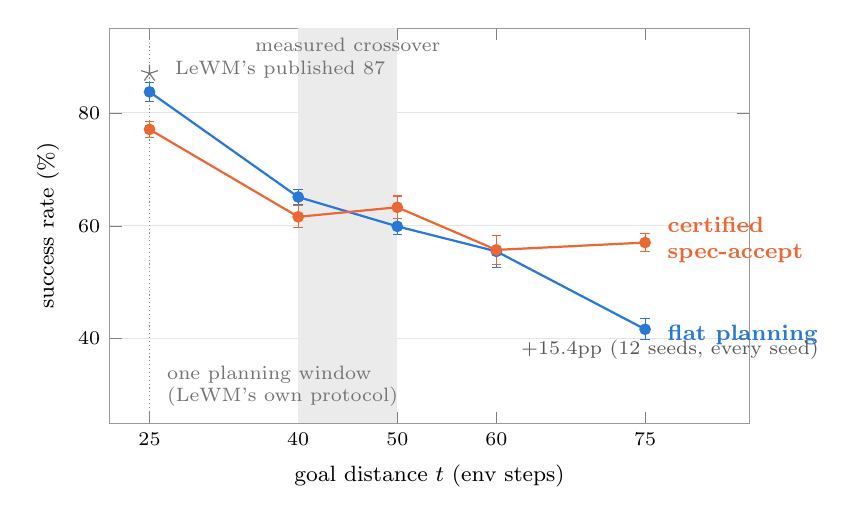
\begin{tikzpicture}
\begin{axis}[
  width=0.8\linewidth, height=6.6cm,
  xmin=21, xmax=85.5, ymin=25, ymax=95,
  xtick={25,40,50,60,75},
  xlabel={goal distance $t$ (env steps)},
  ylabel={success rate (\%)},
  tick label style={font=\scriptsize},
  label style={font=\footnotesize},
  axis line style={black!40},
  ymajorgrids, grid style={black!10},
  clip=false,
]
% measured crossover band [40,50]
\fill[black!8] (axis cs:40,25) rectangle (axis cs:50,95);
\node[font=\scriptsize, color=black!55] at (axis cs:45,92.0)
  {measured crossover};
% one planning window (their protocol) marker
\draw[black!45, densely dotted] (axis cs:25,25) -- (axis cs:25,95);
\node[font=\scriptsize, color=black!55, align=left, anchor=south west]
  at (axis cs:25.8,26.3) {one planning window\\(LeWM's own protocol)};
% LeWM's published Fig. 6 number
\addplot[only marks, mark=star, mark size=3.2pt, black!55]
  coordinates {(25,87)};
\node[font=\scriptsize, color=black!55, anchor=west] at (axis cs:26.6,87.6)
  {LeWM's published 87};
% flat planning (12 seeds; 6 at t=60)
\addplot[gapopen, thick, mark=*, mark size=1.7pt,
         error bars/.cd, y dir=both, y explicit]
  coordinates {
    (25,83.72) +- (0,1.67)
    (40,65.10) +- (0,1.36)
    (50,59.90) +- (0,1.44)
    (60,55.47) +- (0,2.87)
    (75,41.67) +- (0,1.83)};
% certified spec-accept (12 seeds; 6 at t=25 and t=60)
\addplot[gapmech, thick, mark=*, mark size=1.7pt,
         error bars/.cd, y dir=both, y explicit]
  coordinates {
    (25,77.08) +- (0,1.38)
    (40,61.59) +- (0,1.93)
    (50,63.28) +- (0,1.99)
    (60,55.73) +- (0,2.63)
    (75,57.03) +- (0,1.65)};
% direct series labels
\node[gapopen, font=\footnotesize\bfseries, anchor=west]
  at (axis cs:76.3,40.6) {flat planning};
\node[gapmech, font=\footnotesize\bfseries, align=left, anchor=west]
  at (axis cs:76.3,57.5) {certified\\spec-accept};
% headline margin annotation
\node[font=\scriptsize, color=black!65, align=left, anchor=west]
  at (axis cs:61.5,38.0) {$+15.4$pp (12 seeds, every seed)};
\end{axis}
\end{tikzpicture}
\caption{\textbf{TwoRoom on LeWM: the crossover the window rule predicted.} Best
flat and best certified spec-accept arm per goal distance (error bars $=$ SE;
$12$ seeds per point except the declared six-seed cells: both arms at $t{=}60$
and the certified arm at $t{=}25$, whose pooled twelve-seed value, $76.95$,
agrees within $0.2$pp). The $t{=}25$ point is LeWM's published protocol,
star $=$ their Fig.~6 number. The crossover lands in the shaded band $[40,50]$,
inside the frozen prediction; the deployed composite plays flat left of it and
certified spec-accept right of it, and never loses to flat at any measured
horizon.}
\label{fig:tworoom-crossover}
\end{figure}


\paragraph{OGBench-Cube (manipulation): a measured boundary of the threshold rule.}
Cube is the intended out-of-sample test of the \emph{whole} recipe, goal-free
drafter (expert, goal-directed data, the PushT regime), $S{=}10$ zero-shot, and $\tau$
derived from the encoder's criterion floor on an encoder never seen during
calibration. The port reproduces the pipeline (baseline flat planning solves the
single-cube task; encoder and closed loop wire through the benchmark's own $0.04$m
success check), and the $k$-derivation transfers cleanly. The \emph{threshold}
derivation, however, hits a boundary we report rather than paper over: Cube's success
criterion constrains only the cube position, while the encoder observes the whole
scene including the arm. The criterion-floor measurement therefore pairs frames whose
cube matches but whose arm pose does not, inflating the measured floor by
${\sim}10\times$ (p50 $0.97$ vs.\ a normal per-step temporal floor of $0.087$, in line
with PushT's $0.080$). Tightening the equivalence to a \emph{full-scene} match, cube
\emph{and} end-effector, both at the $0.04$m benchmark scale, only partly recovers it
(floor p50 $0.79$, still ${\sim}9\times$ the temporal floor): the encoder retains
substantial visually-salient, task-irrelevant scene variation that no success-based
equivalence pins down. The criterion-floor rule for $\tau$ is thus well-posed only when
the success criterion covers the observed scene; under a \emph{partial}-observation
criterion it is out of scope, and a scope guard (criterion floor within $3\times$ the
temporal floor, else fall back to the transferred default $\tau{=}0.20$) selects the
threshold basis automatically. This is a scope result for the \emph{derivation}, not a
failure of spec-accept, which is threshold-parameterized regardless; the battery ran
the recipe at the transferred-default $\tau$ with the (in-scope) derived $k$, which, applied derive-first to the cube drafter, named $k{=}3$; the closed-loop sweep
run \emph{afterwards} confirms $k{=}3$ as the strongest cell ($81.3$ vs.\ $78.9$ at
$k{=}8$), the derivation rule's second prospective hit.

\paragraph{Cube results: a confirmed win, and one honest miss of the regime map.}
The certified protocol anchors first (flat RH$=$5 reproduces LeWM's published $74\%$
at $71.1$; \Cref{tab:cube}). The regime map's inferability leg then takes its one
loss: \emph{goal-free} drafting fails outright ($33.0$ every-step, $27.3$
spec-accept) despite expert, goal-directed data with a rendered target, the
prediction was that expert data suffices, and it does not; goal-conditioning recovers
$+43$pp on its own ($76.8$, no gating). The failure mechanism is the same overshoot
that bounds short-range Reacher: the drafter, trained on always-in-motion expert
segments, cannot emit ``arrive and stop,'' and the certified task is goal-near
(delivery ${\sim}40$ steps, then a long hold), an arrival gate alone recovers
$+32$pp on the goal-free drafter, and PushT, whose expert episodes \emph{end} at the
goal, is the natural experiment for why it never needed one. With conditioning and
arrival handling the recipe beats flat decisively and approaches the true-waypoint
oracle ($82.4$). All of this then survives the strict test: on eight \emph{fresh}
seeds with the bar frozen in advance ($\ge$ flat $+5$pp), the gated arm confirms at
$+10.5$pp, the exploratory margin ($+10.3$) reproduced on disjoint seeds, and
the $c^{*}$ arbiter (\Cref{sec:method-arbiter}), whose retirement rule replaces the
latent-distance gate, lands \emph{above} it at $79.9$ ($+14.0$ over flat), the
environment's best confirmed number. A decomposition control closes the last
alternative reading: flat at the arbiter's own short window and certified budget
scores only $63.8$, so the win is selection $+$ drafting, not an underrated flat
configuration. One scope nuance is reported rather than smoothed over: on Cube,
$c^{*}$ fires at the first replan on ${\sim}55\%$ of episodes ($c^{*}$ p50
$0.14$--$0.18$) although the physical transport far exceeds the planning window, under a partial-observation criterion the certificate inherits the planner's optimism
toward the goal latent and reads as a per-episode \emph{solvability} signal rather
than literal reachability. The per-episode trace decomposition (pooled, $8$ seeds)
shows that signal is doing real work, the certificate stratifies episodes into a
solvability ladder: episodes retired at the \emph{first} replan succeed at $95.5\%$
($57\%$ of episodes), episodes that draft and then retire on certified arrival at
$75.4\%$ ($33\%$), and the never-retired tail at $9.3\%$ ($10\%$), the genuinely
unsolvable residue, correctly identified by the one signal without any horizon or
task knowledge. We state the instrument's semantics per regime rather than claim
more. Multi-cube (double/triple) remains the genuinely long-horizon manipulation
case and requires that data.

\begin{table}[h]
\centering
\small
\caption{OGBench-Cube, certified protocol (goal offset $150$, budget $300$,
$600$-sample CEM, $n{=}128$/seed; success $=$ cube within $0.04$m). Top:
development seeds (the arms explored there). Bottom: the pre-registered
confirmation on eight fresh seeds (bar frozen in advance: recipe $\ge$ flat
$+5$pp, met at $+10.5$ and $+14.0$). Margins are stable across seed sets;
absolutes move with the population and are never compared across blocks.}
\label{tab:cube}

\vspace{2pt}
\textbf{(a) development} \quad \emph{4 seeds}

\vspace{2pt}
\begin{tabular}{lc}
\toprule
flat (goal image), RH$=$5                    & 70.9 \\
goal-free every-step ($k{=}50$)              & 33.0 \\
goal-free spec-accept                        & 27.3 \\
goal-cond.\ spec-accept (no gate)            & 76.8 \\
goal-cond.\ spec-accept $+$ arrival gate, $k{=}3$ & \ours{81.3} \\
\midrule
oracle (true waypoints)                      & 82.4 \\
\bottomrule
\end{tabular}

\vspace{8pt}
\textbf{(b) pre-registered confirmation} \quad \emph{8 fresh seeds}

\vspace{2pt}
\begin{tabular}{lc}
\toprule
flat (goal image), RH$=$5                    & 65.9 \\
flat, RH$=$2 (arbiter's window; control)     & 63.8 \\
goal-cond.\ spec-accept $+$ arrival gate, $k{=}3$ & 76.5 \\
certified spec-accept (\Cref{sec:method-arbiter}) & \ours{79.9} \\
\bottomrule
\end{tabular}
\end{table}

% ============================================================

\section{Efficiency: Full Accounting}\label{app:eff}

\begin{figure}[h]
\centering
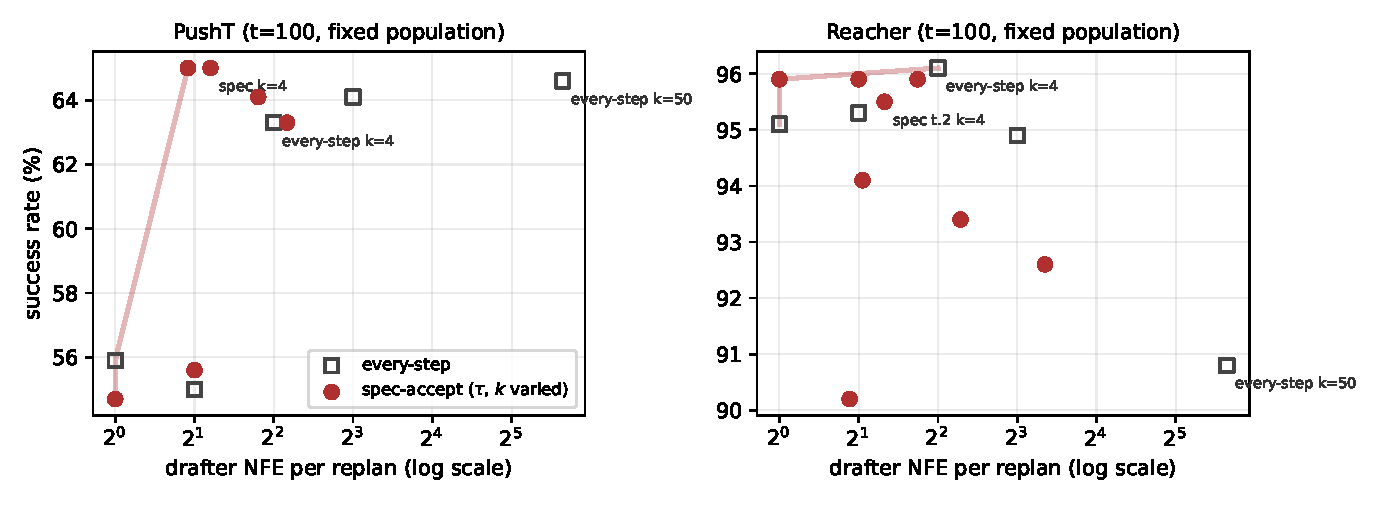
\includegraphics[width=\linewidth]{figs/pareto}
\caption{SR vs.\ drafter compute, every arm on one fixed population per environment
($t{=}100$, $n{=}512$/cell; NFE/replan $=$ call ratio $\times k$). Squares:
every-step drafting across $k$; circles: spec-accept across $\tau$ and $k$; the
frontier is drawn. \textbf{PushT: spec-accept at the frozen config Pareto-dominates}
(higher SR than the $k{=}50$ reference at ${\sim}22\times$ less compute, and than
matched-$k$ every-step at ${\sim}1.7\times$ less). \textbf{Reacher: the frontier is
shared}, cheap every-step drafting is itself strong ($k{=}1$ works), and
spec-accept's marginal factor is ${\sim}1.5\times$ at SR-parity. The $k{\leq}2$ cliff
(PushT, bottom-left) is a consumption-policy artifact, not unusable drafts:
committed blocks at $k{=}2$ recover plateau SR at $1$ NFE/replan
(\Cref{sec:why-verifier}), while $\tau$-verification there falsely rejects
(sampler noise exceeds the floor, \Cref{sec:calib-k}) and inherits every-step's
re-draft churn. The derived $k$ rule keeps the operating point off this cliff.}
\label{fig:pareto}
\end{figure}

At the frozen configuration, spec-accept is SR-neutral or better in every cell of
every regime on both dev environments (call ratios $0.46$--$0.88$), with zero
re-tuning across environments and across goal-free/goal-conditioned drafters
(\Cref{fig:pareto}). Cost, stated as the two factors of \Cref{sec:method-config}:
cheap drafts take the reference from $1500$ to $90$ NFE/episode on their own;
verified consumption removes a further ${\sim}40\%$ of calls at matched $k$, landing
at $1.9$--$2.4$ NFE/replan at the derived configuration.

\paragraph{Why NFE is the right currency.} Measured with CUDA-synced
instrumentation, the drafter is $1.0\%$ of episode wall-clock at $k{=}50$ and $0.4\%$
at the frozen configuration in \emph{this} stack; CEM over an 18M-parameter
dynamics model dominates, and we state that plainly rather than let a wall-clock
number imply otherwise. Drafter NFE is nevertheless the quantity worth optimizing,
for three reasons. First, it is the component that scales: the controller's cost is
fixed by its sample budget and a small dynamics model, while the drafter tier is
where model capacity grows, the same consumption policy applied to a video-scale
drafter inherits the full reduction, and there the drafter \emph{is} the wall-clock.
Second, the factors compose: cheap drafts ($k$) and verified consumption (call ratio)
multiply into any stack with a diffusion proposer, independent of what surrounds it, including stacks whose controller has been distilled or amortized away, where
drafter calls are all that remains. Third, the recipe is wall-clock non-regressive
even here: verification adds no measurable time ($0.4\%$ at $k{=}8$ with or without
spec-accept), and the fine stride it enables runs $12\%$ \emph{faster} end-to-end
than the native configuration at matched protocol. The claim we make is a
drafter-side compute claim, stated with its denominator; the claim we do not make is
an end-to-end latency win on this benchmark.

\paragraph{The arbiter's measured overhead.} The same instrumentation prices the
$c^{*}$ arbiter (PushT $t{=}100$, all-drafting regime, per episode): the derived-$k$
drafter costs $7.9$ms against the controller's $1{,}936$ms ($0.4\%$, drafting is
essentially free at $k{=}3$), and the per-replan retire probe brings certified
spec-accept to $3{,}070$ms, $1.58\times$ the fixed-arm wall-clock, below the $2\times$
bound because the probe plans a shorter window than the policy's own solve. The
asymmetry is the point: at $t{=}25$, where most episodes are certified easy at the
first replan, certified spec-accept completes in $430$ms/episode, cheaper than any
fixed arm, with zero drafter calls on routed episodes by construction. For
reference, the FF-JEPA arms measure $1{,}949$ms ($S{=}10$ loop) and $2{,}449$ms
(native $S{=}25$/RH$=$5) per episode at $2$--$3\%$ drafter share: spec-accept is
wall-clock \emph{ahead} of the published configuration ($-21\%$) at $+2.4$pp SR, and
certified spec-accept costs $1.25\times$ the published configuration for $+2.8$pp. If
the overhead ever matters, the probe admits a knob-free reduction (evaluate $c^{*}$
only at re-draft boundaries, where a solve is being paid for anyway); we report the
conservative every-replan variant throughout. The headline cost figure and its
three readings are in the main text (\Cref{sec:results-eff}, \Cref{fig:cost}).

\section{Negative Results and Ablations}
\label{sec:negatives}
Every alternative we measured loses to the recipe, and each loss confirms one of the
two mechanisms of \Cref{sec:why}. \emph{Spread is load-bearing:} refinement head
$-11$pp, blind commit-3 $-18$pp, learned-confidence adaptive commit worse than blind,
deterministic regressor $-4.4$ to $-11.7$pp at matched offline fidelity. \emph{The
verifier must be reality, not a heuristic:} a goal-gated variant (serve the goal
image whenever a waypoint fails a latent goal-progress test, one greedy attempt to
automate the regime rule inside the verifier) collapses the Reacher long-horizon
advantage from $94.5/93.9$ back toward the flat baseline ($82.8$ at $t{=}100$, $80.1$
at $t{=}150$; call ratio ${\sim}0.8$), while remaining harmless where drafting had no
edge anyway ($91.6$ at $t{=}25$). The matched-$k$ blind-commitment cells of
\Cref{sec:why-verifier} complete the picture: blindness is not uniformly wrong, it ties where verification is idle, but it fails unsignaled in both directions
(depth-3 on PushT, any depth on Reacher), which is precisely what a measured
threshold buys over a commitment ladder.

\begin{table}[h]
\centering
\small
\setlength{\tabcolsep}{5pt}
\caption{Negative results, every alternative to the recipe, grouped by the mechanism
each confirms (controlled protocols; \degc{20} / joint criterion). Every operator that
narrows the drafter's conditional spread toward its mean, or replaces the reality
verifier with a proxy, loses, despite equal-or-better \emph{offline} fidelity in the
spread rows. $\Delta$ is versus that block's reference. The goal-gated row is
diagnosed, not merely reported: latent distance to the goal saturates beyond one hop
(\Cref{sec:calib-tau}), so the gate fires on noise at range and collapses the
long-horizon advantage, while the \emph{same} gating idea, applied where distances
are informative (arrival on Cube, \Cref{tab:cube}), recovers $+32$pp. The $c^{*}$
arbiter (\Cref{sec:method-arbiter}) replaces the saturating instrument with the
planner's certificate and recovers both regimes at once
(\Cref{sec:results-unified}).}
\label{tab:negatives}
\begin{tabular}{llcc}
\toprule
mechanism & arm & SR & $\Delta$ \\
\midrule
\multirow{5}{*}{\shortstack[l]{spread is\\load-bearing}}
 & GDM every-step (PushT reference)          & 91.9 & ref. \\
 & $+$ refinement head (halves offline err.) & 81.1 & $-10.8$ \\
 & $+$ blind commit-3                         & 73.8 & $-18.1$ \\
 & $+$ learned-confidence adaptive commit     & 64.5 & $-27.4$ \\
 & deterministic regressor (matched offline)  & \multicolumn{2}{c}{$-4.4$ to $-11.7$} \\
\midrule
\multirow{2}{*}{\shortstack[l]{verify vs.\\reality}}
 & spec-accept (Reacher long, reference)      & 94.5\,/\,93.9 & ref. \\
 & goal-gated verifier (learned proxy)        & 82.8\,/\,80.1 & $-11.7$\,/\,$-13.8$ \\
\midrule
\multirow{2}{*}{\shortstack[l]{blindness\\unsignaled}}
 & blind commit-2, PushT (verify idle here)   & 65.3 & $+0.3$ \\
 & blind commit-3, Reacher (any depth)        & 87.9\,/\,89.8 & $-6.6$\,/\,$-5.9$ \\
\bottomrule
\end{tabular}
\end{table}

\Cref{tab:negatives} collects them. The dose-response of \Cref{sec:why-spread} is the
continuous version of the top block, and the $\gamma$-sweep's interior optimum at
native spread is what makes ``narrow the spread'' predict a loss in both directions.

% ============================================================

\section{Faithful Reproduction and Audit}
\label{app:repro}
Every number in this paper is produced by a pipeline rebuilt end-to-end from public
assets on independent hardware. Faithfulness is over-determined. A from-scratch rebuild
of the dense training set reproduces the original training population to the episode
($9{,}094$) and the optimizer to the iteration ($171{,}940$); the retrained $S{=}25$
drafter reproduces the reference offline-fidelity anchor to four decimals ($0.1593$
vs.\ $0.1593$ at $m{+}1$); and the closed-loop anchor cells reproduce the original
system within noise (baseline $94.6$ / oracle $92.6$ / $S{=}25$ $94.8$ / $S{=}10$
$99.4$ \degc{20}, against the box-era $93.4/93.4/95.3/98.4$). Offline drafter
diagnostics are not comparable across dense-file rebuilds; the closed-loop anchors are
the arbiter.

\paragraph{Statistical conventions and scope.} Every quoted cell pools $64$--$128$
episodes per seed over $4$--$12$ evaluation seeds ($384$--$1536$ episodes; grid
confirmations at $1024$/cell), with margins tested paired per-seed wherever seeds
match. For calibration, the substrate's own paper \citep{lewm} evaluates $50$
trajectories per published bar and reports training-seed variance ($3$ retrainings)
for one environment; in the single place that convention binds, the Two-Room anchor
replication, we ran their protocol verbatim \emph{including} $n{=}50$.\footnote{One
released-vs-text discrepancy, resolved in the data's favor: their paper text states
$10$ CEM iterations outside PushT while their released configuration specifies $30$;
we follow the released configuration, which is the one that reproduces their
published Two-Room number.} Our seeds are \emph{evaluation} seeds (episode sampling
and CEM) on the frozen released checkpoint: substrate training variance is
deliberately out of scope, since the method takes the stack as given and the
released weights are what makes anchor comparisons faithful. Generality beyond this
checkpoint is tested on a stronger axis instead, across architectures
(\Cref{sec:generality}).

\paragraph{The \degc{20}/\degc{5} criterion.} FF-JEPA's prose states a \degc{5} angular
tolerance, but the environment's shipped evaluation code enforces \degc{20}; the oracle
(true goal, exact pipeline) reaches only ${\sim}84$--$86\%$ at literal \degc{5} even
under matched-population filtering, making a genuine $96\%$ at \degc{5} for a
\emph{sampled}-subgoal method implausible. We treat \degc{20} as the operative
criterion (it is what the code enforces and what every published number matches) and
\degc{5} as a strict precision criterion, reporting both throughout.

\paragraph{Protocols.} \emph{Paper protocol}: $n{=}256$, paper-matched sampling
(reproduction, random-init, and the FF-JEPA-config comparison rows). \emph{Controlled
protocol}: fixed held-out episodes, budget $2t$, block-only criterion, CEM seeds
matched byte-for-byte across arms so within-table deltas are exact treatment effects;
per-arm $\mathrm{SE}\approx1.7$pp (4 seeds) / $0.9$pp (8 seeds). Horizon sweeps use one
fixed episode population per environment, identical episodes at every offset; the two
Reacher populations (max-offset-100 / -150) and the PushT success-filtered /
unfiltered populations are never spliced. Confirmation populations use fresh builder
seeds disjoint from every analysis population ($777$ for gate v3, $888$ for the v4
exploratory run, $999$ for the v4 confirm); seed extensions to $1024$
episodes/cell were declared before their results and pooled without selection.

\begin{table}[h]
\centering
\small
\setlength{\tabcolsep}{4pt}
\caption{Per-environment protocols (every closed-loop cell in the paper).}
\label{tab:protocols}
\footnotesize
\begin{tabular}{lp{2.2cm}p{2.4cm}p{3.0cm}p{2.85cm}}
\toprule
& PushT & Reacher & OGBench-Cube & TwoRoom \\
\midrule
success criterion & block pose, \degc{20} (\degc{5} strict) & all joints within $0.05$\,rad & cube within $0.04$\,m of target & agent within $16$\,px of target \\
episodes/cell & $256\times4$ seeds & $128\times8$ seeds & $128\times8$ seeds (confirm) & $64\times12$ seeds ($64\times6$ crossover interior) \\
budget & $2t$ & $2t$ & $300$ at offset $150$; $600$-sample CEM & $2t$ anchored; $50$ at their $t{=}25$ \\
populations & success-filtered $+$ unfiltered fixed & max-offset-$100$/$150$ $+$ confirm (seed $999$) & holdout episodes ${\ge}8000$, per-seed sampling & unfiltered, holdout ${\ge}4000$; goal from proprio \\
drafter & goal-free, $S{=}10$ & goal-cond., $S{=}10$ & goal-cond., $S{=}10$ & goal-cond.\ paired ($192{+}384$-d), $S{=}10$ \\
$k$ / $\tau$ & $3$ (derived) / $0.20$ (derived) & $8$ (rule: any) / $0.20$ (in-band) & $3$ (derive-first) / $0.20$ (transferred; scope guard) & $50$ ($k$-rule refuted here) / $0.098$ (derived in DINOv2) \\
\bottomrule
\end{tabular}
\end{table}

\section{Controls and Full Grids}
\label{app:controls}
The following controls are summarized in the main text and reported in full here (all
exist in the run logs; provenance in the supplementary).
\begin{itemize}[itemsep=1pt,topsep=2pt]
\item \textbf{Cadence isolation} (\Cref{sec:method-scale}): re-anchoring every $5$ steps
against \emph{unchanged} $25$-step targets collapses SR to $78.6/77.8$ ($-12.5$pp), the mechanism is scale matching, not replan frequency.
\item \textbf{Full $\tau{\times}k$ grid} behind \Cref{fig:pareto}, both environments,
with call ratios; the frozen cell and the $k$-cliff are read off it.
\item \textbf{Replan-rate (RH) sweeps} for the flat baseline, both environments: RH is a
brittle short-vs-long trade-off (Reacher RH$1/2/5$ at $t{=}25$: $91.6/95.7/83.2$; at
$t{=}150$: $46.1/62.3/76.0$), so every comparison anchors to the strongest flat
configuration per cell; no RH rescues flat planning from the horizon collapse.
\item \textbf{Fixed-population horizon tables} at both success-filtered and unfiltered
populations (PushT), reported separately, same qualitative story at different absolute
levels.
\item \textbf{VLWM \citep{vlwm} fixed-budget-50 cross-paper cell}: budget starvation reproduces the
published collapse and inverts the drafting/flat ordering (imperfect waypoints need
budget headroom); cited as ``same budget regime,'' not a like-for-like win.
\item \textbf{Failure anatomy} ($S{=}10$, 8 seeds): $18$ failures in $496$ episodes, all
tolerance-boundary near-misses (final distance within the success distribution's 95th
percentile); zero unreachable-subgoal, divergence, or stuck episodes; FF-JEPA's own
reported failure mode is eliminated at fine scale.
\end{itemize}

\end{document}
